\chapter{Diseño de la solución}
\label{chap:diseño}
\section{Especificación de requisitos}
\label{section:especificación}

\subsection{Historias de usuario (HU)}
Una vez se ha analizado el problema y se han detectado las oportunidades de mejora, se deben definir las características y funcionalidades que se implementarán en la herramienta. A partir de las historias de usuario, que han sido recopiladas y refinadas a través de sesiones de trabajo colaborativas y entrevistas con los investigadores expertos en el dominio, utilizando técnicas de lluvia de ideas para explorar los diferentes escenarios de uso, se van a extraer los criterios de aceptación para verificar que la funcionalidad se define acorde a la idea inicial de los usuarios. Posteriormente, sobre esta base se formulan los requisitos funcionales y no funcionales que estructuran, de una forma detallada, los aspectos o funcionalidades que debe implementar la plataforma.


\renewcommand{\arraystretch}{1.3}
\begin{longtable}{ p{1cm}  p{2.3cm}  p{5cm}  p{5cm} }
\caption{Historias de usuario HU01–HU11} \label{tab:historias-usuario} \\
\toprule
\textbf{ID} & \textbf{Nombre} & \textbf{Historia de usuario} & \textbf{Criterio de aceptación} \\
\toprule
\endfirsthead

\multicolumn{3}{l}{\footnotesize Continues from previous page} \\
\toprule
\textbf{ID} & \textbf{Nombre} & \textbf{Historia de usuario} & \textbf{Criterio de aceptación} \\
\midrule
\endhead


\bottomrule
\multicolumn{3}{l}{\footnotesize Continues on the next page} \\
\endfoot

\bottomrule
\endlastfoot

HU01 & Inicio de sesión & Como usuario de la aplicación, quiero poder iniciar sesión con mis credenciales, para acceder de forma segura a mi cuenta personal y a todos mis análisis. & Dado que estoy en la pantalla de inicio de sesión, cuando introduzco mis credenciales y presiono el botón de inicio de sesión, entonces me muestra los análisis que he hecho previamente. \\
\midrule
HU02 & Panel de control & Como usuario de la aplicación, quiero tener acceso a un panel de control centralizado, para visualizar de un vistazo el estado y progreso de todos mis análisis PRS pendientes y completados. & Dado que he iniciado sesión, cuando entro a la pantalla principal de la \textit{app}, entonces se muestra un panel con los estados y progreso de todos mis análisis. \\
\midrule
HU03 & Crear nuevo análisis PRS & Como usuario de la aplicación, quiero crear un nuevo análisis PRS para estimar la predisposición genética a enfermedades específicas de mis pacientes. & Dado que estoy en la pantalla principal, cuando presiono el botón de nuevo análisis, entonces me lleva a la pantalla de creación de análisis PRS. \\
\midrule
HU04 & Gestión de análisis PRS & Como usuario de la aplicación, quiero gestionar mis análisis PRS, para visualizar, ordenar o eliminar estudios según necesite. & Dado que he iniciado sesión y estoy en el panel de control, cuando selecciono un análisis, entonces me muestra opciones de visualizarlo, ordenarlo o eliminarlo. \\
\midrule
HU05 & Subida de archivos genéticos & Como usuario de la aplicación, quiero subir archivos \textit{VCF/PLINK1/PLINK2/23andME}, para utilizarlos posteriormente en los análisis de PRS. & Dado que estoy en la pantalla de creación de análisis PRS, cuando presiono el botón para cargar \textit{datasets}, entonces me deja seleccionar mis propios \textit{datasets} en formato \textit{VCF/PLINK1/PLINK2/23andME}. \\
\midrule
HU06 & Selección de modelos PRS & Como usuario de la aplicación, quiero seleccionar una agrupación de modelos PRS para aplicarlos al paciente. & Dado que estoy en la pantalla de creación de análisis PRS, cuando selecciono uno o varios modelos de la lista, entonces me deja asignarlos a mi análisis. \\
\midrule
HU07 & Configuración del análisis PRS & Como usuario de la aplicación, quiero configurar los parámetros del análisis PRS, para personalizar el estudio. & Dado que estoy en la pantalla de creación de análisis PRS, cuando selecciono y ajusto diferentes parámetros, entonces se quedan guardados y me deja ejecutar el análisis con ellos. \\
\midrule
HU08 & Ejecución del análisis & Como usuario de la aplicación, quiero iniciar un análisis de PRS con un solo clic después de la configuración, para obtener resultados sobre la predisposición genética de mis pacientes. & Dado que ya he configurado mi análisis, cuando presiono el botón de iniciar análisis, entonces la \textit{app} empieza la ejecución de mi análisis PRS, mostrando su progreso. \\
\midrule
HU09 & Visualización de resultados & Como usuario de la aplicación, quiero visualizar los resultados para facilitar la interpretación del riesgo de mis pacientes. & Dado que un análisis ha finalizado y en la pantalla se muestra como completado, cuando lo selecciono y le doy al botón de ''\textit{view}'', entonces me muestra una pantalla con el resultado. \\
\midrule
HU10 & Exportación de resultados & Como usuario de la aplicación, quiero exportar los resultados para incluirlos en otros sistemas. & Dado que un análisis ha finalizado y en la pantalla se muestra como completado, cuando lo selecciono y le doy al botón de exportar, entonces, se genera y exporta en formato PDF. \\
\midrule
HU11 & Notificaciones al finalizar análisis & Como usuario de la aplicación, quiero recibir notificaciones cuando se complete un análisis, para gestionar eficientemente mi tiempo. & Dado que he ejecutado un análisis, cuando este finaliza, entonces recibo una notificación en el correo y un \textit{pop-up} en la \textit{app} avisando que el análisis ha concluido. \\

\end{longtable}

A partir de los criterios de aceptación formulados, se han definido los siguientes requisitos funcionales y no funcionales, los cuales se clasifican a su vez por nivel de prioridad.

\subsection{Requisitos funcionales (RF)}

 A partir de los criterios de aceptación de las historias de usuario, se han derivado los requisitos funcionales (RF). Estos requisitos traducen las necesidades del usuario en especificaciones concretas sobre lo que el sistema debe hacer. Describen las funciones, tareas y comportamientos específicos que la plataforma debe ser capaz de ejecutar para satisfacer las historias de usuario definidas.

\renewcommand{\arraystretch}{1.3} % más espacio entre filas
\begin{longtable}{ p{1.2cm}  p{2cm}  p{3.5cm}  p{1.5cm}  p{2.2cm}  p{1.9cm} }
    \caption{Requisitos funcionales RF-001 – RF-019} \label{tab:requisitos-funcionales} \\
    \toprule
    \textbf{ID} & \textbf{Nombre} & \textbf{Descripción} & \textbf{Prioridad} & \textbf{Dependencias} & \textbf{Historia de usuario} \\
    \toprule
    \endfirsthead

    \multicolumn{3}{l}{\footnotesize Continues from previous page} \\
    \toprule
    \textbf{ID} & \textbf{Nombre} & \textbf{Descripción} & \textbf{Prioridad} & \textbf{Dependencias} & \textbf{Historia de usuario} \\
    \midrule
    \endhead

    \bottomrule
    \multicolumn{3}{l}{\footnotesize Continues on the next page} \\
    \endfoot
    
    \bottomrule
    \endlastfoot

    RF-001 & Inicio de sesión & El sistema debe permitir a los usuarios iniciar sesión con sus credenciales. & Media & -- & HU01 \\
\midrule
    RF-002 & Panel de control & El sistema debe proporcionar un panel de control de estados de sus análisis. & Alta & RF-001 & HU02 \\
\midrule
    RF-003 & Organización de los análisis & Los análisis deben estar organizados de forma clara. & Media & RF-002 & HU02 \\
\midrule
    RF-004 & Creación de análisis & El sistema debe permitir la creación de un nuevo análisis PRS desde el panel de control. & Alta & RF-002 & HU03 \\
\midrule
    RF-005 & Filtro de los análisis & El sistema debe permitir filtrar los análisis según diferentes criterios, como fecha de creación, estado, tipo de análisis... & Media & RF-003 & HU02 \\
\midrule
    RF-006 & Búsqueda entre los análisis & El sistema debe proporcionar una barra de búsqueda para localizar análisis por nombre, ID o palabras clave. & Alta & RF-002 & HU02 \\
\midrule
    RF-007 & Visualización de los detalles del análisis & El usuario debe poder visualizar la configuración, descripción y modelos que componen el análisis accediendo con un botón desde el panel de control. & Alta & RF-002 & HU04 \\
\midrule
    RF-008 & Eliminación de análisis & El sistema debe permitir a los usuarios eliminar análisis PRS. La eliminación debe requerir confirmación. & Media & RF-002 & HU04 \\
\midrule
    RF-009 & Selección de modelos & El sistema debe permitir seleccionar modelos PRS predefinidos. & Alta & RF-004 & HU06 \\
\midrule
    RF-010 & Carga de \textit{datasets} (estándar y formato específico) & El sistema debe permitir seleccionar \textit{datasets} predefinidos. & Alta & RF-004 & HU05 \\
\midrule
    RF-011 & Configuración de análisis & El sistema debe permitir configurar parámetros adicionales de los análisis. & Alta & RF-004 & HU07 \\
\midrule
    RF-012 & Estado del análisis & El sistema debe mostrar el progreso de la ejecución del análisis. & Alta & RF-002 & HU08 \\
\midrule
    RF-013 & Cancelación de análisis & El sistema debe permitir a los usuarios cancelar un análisis en ejecución. & Alta & RF-012 & HU08 \\
\midrule
    RF-014 & Visualización de resultados (pantalla) & El sistema debe permitir la visualización de resultados de un análisis PRS. & Alta & RF-012 & HU09 \\
\midrule
    RF-015 & Exportación de resultados & El sistema debe permitir exportar resultados en formato PDF. & Media & RF-014 & HU10 \\
\midrule
    RF-016 & Notificación al usuario & El sistema debe enviar notificaciones a los usuarios cuando un análisis PRS se complete. & Media & RF-012 & HU11 \\
\midrule
    RF-017 & Notificación en la \textit{app} & Al completarse la ejecución de un análisis PRS las notificaciones pueden ser en la \textit{app}. & Media & RF-016 & HU11 \\
\midrule
    RF-018 & Notificación por correo electrónico & Al completarse la ejecución de un análisis PRS las notificaciones pueden ser por correo electrónico. & Baja & RF-016 & HU11 \\
\end{longtable}

\subsection{Requisitos no funcionales (RNF)}

 Complementando a los requisitos funcionales, los requisitos no funcionales (RNF) definen cómo debe operar el sistema. En lugar de describir funciones, especifican los criterios de calidad, las restricciones y las propiedades de la plataforma, como su rendimiento (ej. tiempo de carga), seguridad, usabilidad y escalabilidad. Estos requisitos son cruciales para garantizar que la experiencia del usuario sea satisfactoria y que el sistema sea robusto y fiable.

\renewcommand{\arraystretch}{1.3} % más espacio entre filas
\begin{longtable}{ p{1.5cm}  p{2.2cm}  p{3cm}  p{1.3cm}  p{2.2cm}  p{2cm} }
    \caption{Requisitos no funcionales RNF-001 – RNF-004} \label{tab:requisitos-no-funcionales} \\
    \toprule
    \textbf{ID} & \textbf{Nombre} & \textbf{Descripción} & \textbf{Prioridad} & \textbf{Dependencias} & \textbf{Historia de usuario} \\
    \toprule
    \endfirsthead

    \multicolumn{3}{l}{\footnotesize Continues from previous page} \\
    \toprule
    \textbf{ID} & \textbf{Nombre} & \textbf{Descripción} & \textbf{Prioridad} & \textbf{Dependencias} & \textbf{Historia de usuario} \\
    \midrule
    \endhead

    \multicolumn{3}{l}{\footnotesize Continues on the next page} \\
    \endfoot

    \bottomrule
    \endlastfoot

    RNF-001 & Seguridad & La autenticación debe tener cifrado seguro. & Alta & RF-001 & HU01 \\
\midrule
    RNF-002 & Tiempo de carga de pantalla & La pantalla principal de la aplicación (panel de control) debe cargar en menos de 2 segundos. & Alta & RF-002 & HU02, HU09 \\
\midrule
    RNF-003 & Valor de rendimiento \textit{Lighthouse} \footnote{Lighthouse es una herramienta destinada a mejorar el rendimiento de las páginas web, ejecutando una serie de auditorías en la página y, luego, generando un informe sobre su rendimiento.} & La aplicación debe obtener una puntuación superior a 90 en \textit{Lighthouse}. & Media & RNF-002 & HU02, HU09 \\
\midrule
    RNF-004 & Interfaz intuitiva & La UI debe ser clara y fácil de usar para que se puedan realizar análisis sin dificultad. & Media & RF-002, RF-003 & HU02, HU09 \\

\end{longtable}

\section{Diseño}
\label{section:diseño}

\subsection{Análisis de posibles soluciones}

En el diseño de la solución se barajan varias alternativas con objeto de facilitar el análisis de PRS a usuarios sin conocimientos técnicos. 

La primera opción consiste en integrar múltiples herramientas ya existentes como \textit{PRSice-2}, el catálogo \textit{PGS} o entornos de visualización como \textit{R/Shiny}; este modelo permite reaprovechar soluciones ya validadas en el ámbito científico. Sin embargo, implica una complejidad técnica elevada para lograr una integración funcional y fluida. El hecho de utilizar herramientas heterogéneas, pensadas para usarse de forma individual, dificulta la cohesión de la solución y añade carga al desarrollo, por lo que se aleja del objetivo principal del proyecto, que es ofrecer una experiencia accesible y sencilla. 

Otra opción que se baraja es la construcción desde cero de una herramienta propia, lo que puede dar completo control sobre el diseño de la interfaz, las funcionalidades y la lógica. A pesar de las ventajas, tiene también dos claros problemas: por un lado, el coste de desarrollarla desde cero y, por otro, hay gran cantidad de funcionalidades iguales o parecidas a las que se busca que tenga la herramienta que ya están resueltas en herramientas existentes. 

Por último, como opción más equilibrada, se plantea usar una herramienta base ya existente y desarrollar una capa de interacción adicional, accesible y amigable al usuario. Se minimiza el desarrollo reutilizando una herramienta ya probada, a la vez que se sigue permitiendo centrarse en la experiencia de usuario a través de una capa de interacción intuitiva y usable. También es técnicamente viable puesto que se separa el cálculo en el \texttt{backend}, reutilizable por otras aplicaciones, y un \texttt{frontend}, para el que se tiene en cuenta principalmente la simplicidad y la usabilidad. Aunque limita un poco debido a que la herramienta base marca la línea a seguir, es la opción escogida si se adapta a los objetivos del proyecto y al usuario final.

\subsection{Solución propuesta}

Finalmente, se ha decidido escoger la última opción y usar \textit{GenoPred} como herramienta base para el desarrollo del sistema. \textit{GenoPred} es una herramienta especialmente diseñada para el cálculo de PRS, que es compatible con los modelos del catálogo \textit{PGS} y que soporta los principales formatos genómicos como \textit{PLINK} o \textit{VCF}. Al mismo tiempo, su punto fuerte es que cuenta con una arquitectura modular basada en reglas, lo que permite ejecutar el \textit{pipeline} rama a rama o todo junto dependiendo de las necesidades. Con \textit{GenoPred} también se pueden analizar individuos concretos, lo cual es muy importante, por ejemplo, en entornos clínicos, donde quizás no se trabaja con ''grandes'' cohortes, además de proporcionar una población de referencia interna, indispensable para poder contextualizar los resultados de los pacientes. 

Otro punto a favor es su compatibilidad con ejecución desde línea de comandos, por lo que resulta fácilmente integrable desde un \texttt{backend}, y su carácter de software libre, su mantenimiento activo y su detallada documentación. A partir de esta base se ha estudiado qué funcionalidades de \textit{GenoPred} implementar en la interfaz web, y se ha decidido apostar por aquellas fundamentales para que cualquier usuario, aunque no tenga grandes conocimientos técnicos, pueda llevar a cabo un análisis PRS completo. Por tanto, se han descartado funciones como la creación de modelos nuevos o la configuración avanzada de pasos intermedios, ya que resultan, en teoría, más complejas para el usuario. En su lugar, se han incorporado funcionalidades como la subida de datos, la selección de modelos ya existentes y la visualización de los resultados, todo ello de un modo guiado y, por tanto, más sencillo de seguir por cualquier usuario. 

Las fases de desarrollo que se van a seguir son:
\begin{enumerate}
    \item \textbf{Desarrollo de la Interfaz de Usuario (\textit{Frontend-First}):}
    Se ha decidido iniciar la implementación desarrollando el diseño de la interfaz de usuario (UI). Esta decisión se justifica por una metodología de diseño centrada en el usuario que permite representaciones tangibles tempranas de las experiencias del usuario.
    
    Esto prioriza los \texttt{front-ends} para recopilar comentarios tempranos sobre la usabilidad y el flujo de trabajo, lo cual es crítico para validar las expectativas del usuario y refinar los requisitos. 
    
    Además de los contratos de UI definidos y una visión clara, el \texttt{backend} solo requiere una eficiencia más dirigida en el desarrollo de \textit{endpoints} y servicios. 
    \item \textbf{Definición e Implementación de la Lógica de \texttt{Backend}:} 
    Inmediatamente después, se procederá a definir e implementar los \textit{endpoints} para la API. Estos \textit{endpoints} serán los enlaces fundamentales para conectar la lógica del \texttt{frontend} con los servicios de procesamiento en el \texttt{backend}. 
    
    El aspecto crucial de esta fase estará vinculado a herramientas computacionales especializadas como \texttt{Genopred}, que está ejecutando el análisis PRS. Debido a la naturaleza CLI de \texttt{Genopred} como una herramienta existente, se ha optado por invocarla a través de un proceso hijo \textit{(child process)}. Esto permite que el servicio de \texttt{backend} (probablemente el \texttt{Orchestrator} o un componente específico de la API) ejecute \texttt{Genopred} como un programa externo, pasando parámetros de entrada a través de la terminal y capturando sus salidas.
    
    La estrategia utiliza la funcionalidad ya bien probada de \texttt{Genopred} sin reimplementar su lógica computacional y, por lo tanto, es sencilla de conectar y menos propensa a errores en el cálculo genético. 
    \item \textbf{Pruebas Exhaustivas y Aseguramiento de la Calidad:}
    La última fase del desarrollo se centrará en la implementación de pruebas extensivas para la validación exhaustiva de la solución. 
    
    Las pruebas unitarias llevarán a cabo verificaciones de que los módulos individuales funcionan bien, las pruebas de integración comprobarán que la comunicación entre los diferentes componentes del sistema (\texttt{Frontend}, API, \texttt{Prisma}, \texttt{Genopred}, etc.) discutidos es correcta y fluida, y las pruebas de extremo a extremo simularán escenarios de uso reales desde la perspectiva del usuario. 
    
    Se hará un énfasis especial en los componentes de importancia funcional: la configuración correcta de los análisis PRS (validando que todos los parámetros se almacenan y recuperan correctamente) y la ejecución precisa de los análisis en \texttt{Genopred} (verificando que los comandos se invocan correctamente, los datos se procesan y los resultados obtenidos cumplen con los requisitos).
    
    El objetivo es asegurar que todas las funcionalidades cumplen con los requisitos funcionales previamente definidos y que la plataforma es estable y fiable. 
\end{enumerate}

%\subsection{Modelado conceptual}
%Para modelar y describir la estructura y el comportamiento del sistema de una forma clara y estandarizada, se ha llevado a cabo un modelado conceptual del sistema. Este proceso sirve como puente entre el análisis del problema y el diseño detallado de la solución, modelando una idea de cómo va a ser el proyecto para la posterior implementación. A continuación, se presentan los artefactos de modelado que definen la arquitectura y el comportamiento del sistema: los diagramas de clases, que establecen la estructura estática del dominio; el diagrama de alto nivel, que describe la arquitectura de componentes; y los diagramas de secuencia, que representann el comportamiento del sistema en los casos de uso principales.

\subsection{Modelo de dominio}
Se va a empezar mostrando el desarrollo del modelo de dominio, representado mediante diagramas de clases UML. El desarrollo de este modelo ha seguido un proceso iterativo que ha permitido asegurar que el modelo final fuera robusto, preciso y proporcionase una representación detallada del dominio. Cada iteración ha sido el resultado de sesiones de trabajo conjuntas entre el equipo de desarrollo y los expertos del dominio, asegurando así que cada versión sea justificada tanto por necesidades técnicas como por una correcta representación del dominio.

Este proceso iterativo se ha llevado a cabo hasta que se ha alcanzado un punto de consenso donde el modelo final ha sido aceptado por ambas partes como una representación fiel del dominio, y ha servido a las necesidades de la implementación de la plataforma.

La primera versión del modelo de dominio (mostrada en la Figura~\ref{fig:clases1}) corresponde al borrador inicial, que surge a partir del conocimiento obtenido durante la fase de la \textit{Investigación del Problema} (sección \ref{chap:investigación}).

Las entidades pertenecientes a esta primera versión son:  

\begin{itemize}
    \item \textbf{\texttt{User}}: Representa al usuario de la plataforma. Contiene los atributos básicos para la autenticación y la gestión de la cuenta, como el \texttt{email} y la \texttt{contraseña}. Es la entidad principal que realiza los análisis.
    
    \item \textbf{\texttt{PRS\_Analysis}}: Es la entidad central del modelo. Contiene toda la información relevante para la configuración y el estado de un análisis, incluyendo su nombre, descripción, el estado actual (ej. en curso, completado) y la ruta al fichero de resultados.
    
    \item \textbf{\texttt{Patient}}: Modela al individuo cuyos datos genómicos se van a analizar. Cada análisis está asociado a un único paciente, almacenando la ruta a su fichero de datos.
    
    \item \textbf{\texttt{PRS\_Model}}: Representa los modelos de Puntuación de Riesgo Poligénico. Almacena metadatos clave sobre cada modelo, como su identificador del catálogo PGS, el nombre y el fenotipo (enfermedad o rasgo) asociado.
    
    \item \textbf{\texttt{Analysis\_Config}}: Esta entidad encapsula los parámetros de configuración específicos de un análisis, como los umbrales de ancestría y de solapamiento. Se vincula a una población de referencia para contextualizar los resultados.
    
    \item \textbf{\texttt{Population}}: Contiene la información sobre las poblaciones de referencia utilizadas para comparar y normalizar los resultados de un análisis.
    
    \item \textbf{\texttt{Result}}: Modela el resultado final de un análisis PRS completado. Almacena la puntuación PRS calculada, el percentil del individuo y un indicador de si el resultado ha sido exportado.
    
    \item \textbf{\texttt{Notification}}: Representa las notificaciones generadas por el sistema para informar al usuario sobre el estado de sus análisis (ej. finalización exitosa o fallo).
\end{itemize}

A partir de estas clases, las relaciones más relevantes de este modelo inicial son:
\begin{itemize}
    \item \textbf{\texttt{User} - \texttt{PRS\_Analysis}}: Un \texttt{User} realiza múltiples \texttt{PRS\_Analysis}. Esta es la relación principal que vincula los análisis a quien los ejecuta.
    
    \item \textbf{\texttt{PRS\_Analysis} - \texttt{Patient}}: Cada \texttt{PRS\_Analysis} se analiza en un único \texttt{Patient}. Esto asegura que cada análisis esté asociado a un individuo concreto.
    
    \item \textbf{\texttt{PRS\_Analysis} - \texttt{PRS\_Model}}: Un \texttt{PRS\_Analysis} incluye uno o varios \texttt{PRS\_Model}, definiendo qué modelos se aplicarán en ese análisis.
    
    \item \textbf{\texttt{PRS\_Analysis} - \texttt{Analysis\_Config}}: Cada \texttt{PRS\_Analysis} tiene una configuración asociada, representada por la entidad \texttt{Analysis\_Config}.
    
    \item \textbf{\texttt{Analysis\_Config} - \texttt{Population}}: La \texttt{Analysis\_Config} hace referencia a una \texttt{Population} para la normalización de los resultados.
    
    \item \textbf{\texttt{PRS\_Analysis} - \texttt{Result}}: Un \texttt{PRS\_Analysis} completado genera un \texttt{Result}. La cardinalidad 0..1 indica que el resultado solo existe si el análisis ha finalizado con éxito.
    
    \item \textbf{\texttt{PRS\_Analysis} - \texttt{Notification}}: Un \texttt{PRS\_Analysis} envía múltiples \texttt{Notifications} al usuario para informarle de cambios de estado.
\end{itemize}

\begin{figure}[H]
    \centering
    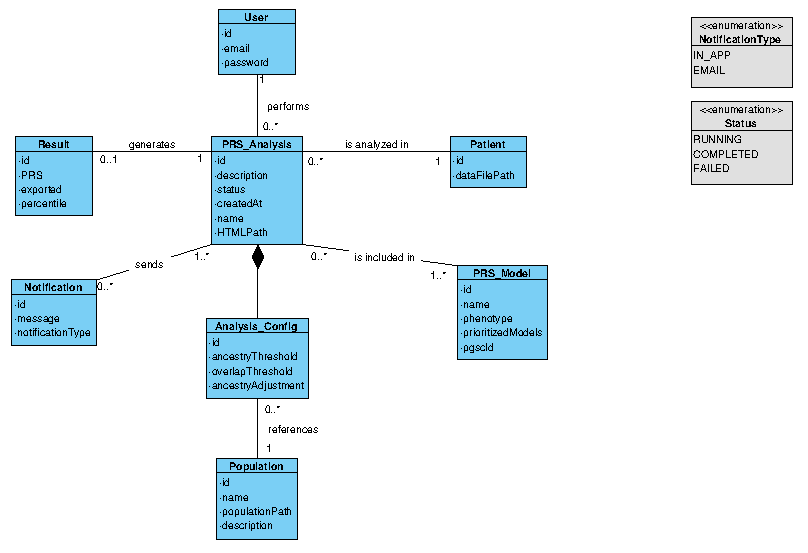
\includegraphics[angle=270, width=1\textwidth]{tfgetsinf/images/Class Diagram0.pdf}
    \caption{Diagrama de Clases v.1}
    \label{fig:clases1}
\end{figure}

Tras una revisión inicial a partir de la presentación del modelo a los tutores y compañeros de trabajo, se identificaron varias áreas de mejora y nuevas necesidades que dieron lugar a una segunda versión del modelo, presentada en la Figura~\ref{fig:clases2}. Esta iteración refina el modelo inicial para representar mejor el dominio y considerar el punto de vista de los expertos. Los cambios han sido los siguientes: 

\begin{itemize} 

    \item \textbf{Eliminación de la clase \texttt{User}:} Para desacoplar el modelo de dominio de la gestión de la autenticación, se eliminó la clase \texttt{User} y se sustituyó por un atributo \texttt{userId} en \texttt{PRSAnalysis}. Esto simplifica el modelo y delega la responsabilidad de la gestión de usuarios a un servicio externo llamado \textit{Auth0}. 

    \item \textbf{Creación de la clase \texttt{PrioritizedModels}:} Para modelar explícitamente la relación entre un análisis y los múltiples modelos PRS que puede utilizar, se extrajo esta lógica a una clase propia, permitiendo tener disponible la lista de los modelos seleccionados en cada análisis. 

    \item \textbf{Adición de \texttt{ScoringFile} y \texttt{Trait}:} Para representar de forma más granular la información de los modelos, se añadieron estas clases que contienen, respectivamente, la ruta al fichero de puntuaciones y los rasgos o fenotipos asociados. 

    \item \textbf{Eliminación de la clase \texttt{Notification}:} Se determinó que las notificaciones son una funcionalidad del sistema y no un concepto central del dominio del problema. Su eliminación del diagrama de clases ayuda a mantener el modelo enfocado en la lógica principal. 

\end{itemize} 

\begin{figure}[H]
    \centering
    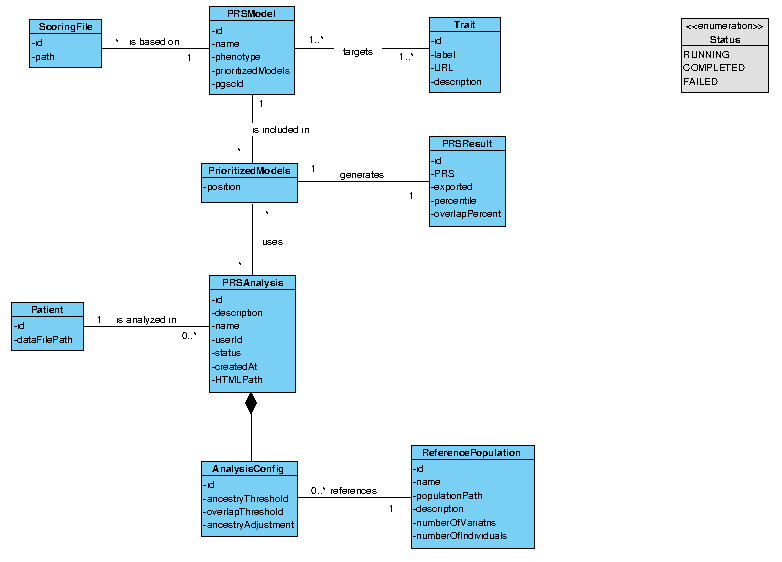
\includegraphics[angle=270, width=1\textwidth]{tfgetsinf/images/Class Diagram1.pdf}
    \caption{Diagrama de Clases v.2}
    \label{fig:clases2}
\end{figure}

Tras una nueva reunión, la validación exhaustiva con los expertos del dominio ha revelado nuevas necesidades y también oportunidades de mejora, que han llevado a una tercera y definitiva versión del diagrama de clases presentado en la Figura~\ref{fig:clases3}. Esta entrega representa la consolidación del modelo de dominio, con un mayor nivel de detalle y avances en las dificultades encontradas para representar el dominio de la forma más robusta y fiable posible y que requieran la plataforma de implementación. 

Los cambios aplicados a la versión anterior han sido los siguientes: 

\begin{itemize}
    \item \textbf{Consolidación de la configuración del análisis en \texttt{PRSAnalysis}}
    La clase antigua \texttt{AnalysisConfig} que se usaba para envolver parámetros como \texttt{ancestryThreshold}, \texttt{overlapThreshold} y \texttt{ancestryAdjustment} ha sido eliminada. Sus características se han incorporado directamente en la clase \texttt{PRSAnalysis}. Estos cambios se han hecho para simplificar el modelo, ya que la forma de configurar un análisis PRS está inherentemente ligada a la instancia del análisis en sí y porque \texttt{AnalysisConfig} no tenía identidad independiente que justificara su existencia como clase separada.
    
    \item \textbf{Enriquecimiento de clases con nuevos atributos:} Para disponer de una representación más completa de los datos y las funcionalidades que requiere la plataforma, se han añadido numerosos atributos a diversas clases ya existentes. 
    
        \begin{itemize}
            \item En \texttt{ReferencePopulation}, se han añadido \texttt{-studyURL} y \texttt{-studyName}, que permiten documentar de dónde vienen las poblaciones de referencia que se usan para analizar los datos y saber cuál es el contexto de ese estudio. Sin esto, no se pueden analizar ni entender los resultados que se obtienen.
            
            \item La clase \texttt{Patient}, se ha enriquecido con \texttt{-genotypingMethod} y \texttt{-DataFileFormat}, que son de ayuda para poder contar cómo se ha obtenido el genotipo de los datos almacenados en la clase \texttt{Patient} y en qué formato está el archivo de entrada. Sin esta información, no existe ni la capacidad de trabajar con estos datos ni de interpretarlos de forma correcta.
            
            \item \texttt{PRSModel} ahora incorpora \texttt{-numberOFSNP}, un atributo esencial para conocer cuántos polimorfismos de nucleótido único (SNPs) forman parte de cada modelo, lo cual da una pista sobre su complejidad y el nivel de detalle de su construcción.
            
            \item La clase \texttt{Trait} ha cambiado con la incorporación de identificadores externos como \texttt{-orphaId}, \texttt{-hpoId}, \texttt{-mondoId}, \texttt{-efoId} y \texttt{-otherId}. Estos IDs estandarizados permiten que los rasgos genéticos se unan a bases de datos y ontologías biomédicas que ya están establecidas (como Orphanet para enfermedades raras, HPO para fenotipos humanos, Mondo para enfermedades...), de esta manera se hace más fácil la interoperabilidad y la integración con otras fuentes de conocimiento genómico.
        \end{itemize}
        
    \item \textbf{Introducción de las clases:} Para reflejar con precisión las nuevas complejidades y los nuevos requisitos del modelo de dominio, se han añadido varias clases nuevas a esta entrega final que enriquecen la capacidad del sistema de describir y hacer su función.
        \begin{itemize}
        \item \texttt{BroadAncestryCategory}: La importancia de la diversidad ancestral en la precisión y aplicabilidad de los Polygenic Risk Scores (PRS) es crucial, es por eso que se ha añadido esta clase. Permite clasificar y gestionar las diferentes categorías de ascendencia relevantes para los modelos PRS y las poblaciones de referencia. Su inclusión es necesaria para asegurar que los análisis puedan ajustar los resultados teniendo en cuenta el contexto ancestral del paciente.
        
        \item \texttt{BroadAncestryInModel}: Es una clase de asociación que surge de la necesidad de cuantificar a modo de porcentaje la contribución o aplicabilidad de una categoría ancestral dada a un modelo, permitiendo así una mayor granularidad en la definición de la composición ancestral de los modelos y su adecuación para diferentes grupos poblacionales.
        
        \item \texttt{BroadAncestryInRefPop}: Esta clase de asociación que es similar a la anterior, se ha introducido para especificar la composición ancestral de una población de referencia concreta. Es esencial para documentar la distribución de las diferentes categorías ancestrales dentro de las poblaciones de referencia utilizadas para la validación de los modelos PRS.
        
        \item \texttt{Publication}: Para establecer un enlace directo y transparente entre los modelos PRS y la literatura científica que los sustenta, se ha incluido esta clase, la cual almacena metadatos clave que permiten acceder rápidamente a la fuente original de la investigación detrás de cada modelo utilizado en los análisis.
        
        \item \texttt{TraitCategory}: Para mejorar la organización y la capacidad de búsqueda de los rasgos genéticos, se ha añadido esta clase, que permite categorizar los \texttt{Trait} de forma jerárquica o temática (''Enfermedades Cardíacas'', ''Trastornos Neurológicos''), facilitando la gestión de rasgos.
        \end{itemize}
\end{itemize}

\begin{figure}[H]
    \centering
    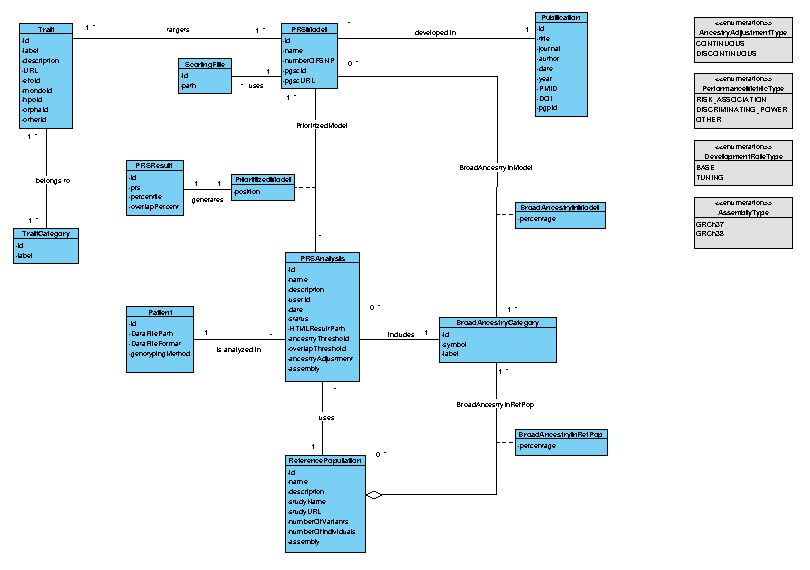
\includegraphics[angle=270, width=1\textwidth]{tfgetsinf/images/Class Diagram2.pdf}
    \caption{Diagrama de Clases v.3}
    \label{fig:clases3}
\end{figure}

\subsection{Diagrama de paquetes}

Para obtener una visión de alto nivel de la estructura del sistema, se ha elaborado un diagrama de paquetes UML, representado en la Figura~\ref{fig:highlevel}. Este tipo de diagrama proporciona una vista macroscópica del sistema, organizando los elementos del modelo en paquetes relacionados para mostrar su estructura y sus dependencias. El uso de este diagrama simplifica la comprensión, la gestión y la comunicación del diseño de un proyecto de software complejo.
En este caso, el diagrama de paquetes organiza la arquitectura de la aplicación en los tres paquetes principales siguientes:

\begin{itemize} 

    \item \textbf{Frontend}: Es la paquete de presentación, responsable de la interfaz de usuario (UI) y la interacción directa con el usuario. Está construida sobre un moderno \textit{framework} de aplicaciones web que permite renderizar las páginas y los componentes visuales. Dentro de esta capa, un componente \texttt{Autenticador} gestiona la lógica del lado del cliente para la autenticación, interactuando con un servicio de identidad externo.

    \item \textbf{Backend}: Es el paquete de lógica de negocio, donde reside el núcleo funcional de la aplicación. La integran los componentes siguientes:

        \begin{itemize} 

            \item \textbf{Capa de API:} Proporciona los \textit{endpoints} de la API \textit{RESTful} a los que el \texttt{frontend} realiza las peticiones. Conecta el \texttt{Frontend} con la capa de acceso a datos y el sistema de ficheros.
            \item \textbf{Orchestrator}: Es el componente central que coordina las operaciones. Gestiona el flujo de creación, ejecución y consulta de los análisis PRS, ya que está directamente ligado al servicio externo \texttt{Genopred}.
            \item \textbf{Capa de Acceso a Datos (ORM):} Actúa como un Mapeo Objeto-Relacional (ORM), facilitando la comunicación con la base de datos de una manera segura y tipada.
            \item \textbf{Notifier}: Gestiona el envío de notificaciones al usuario (ej. por correo electrónico) cuando un análisis finaliza.

        \end{itemize} 

    \item \textbf{Services}: Incluye tanto componentes externos como internos que dan soporte a la aplicación. 

        \begin{itemize} 

            \item \textbf{Servicio de Autenticación y Autorización:} Es un servicio externo de gestión de identidad que se encarga de la autenticación y autorización de usuarios de forma segura.
            \item \textbf{File System}: Representa el sistema de archivos del servidor donde se almacenan temporalmente los datos genómicos de los pacientes y los resultados de los análisis PRS. 
            \item \textbf{Genopred}: Es el motor de cálculo bioinformático. El \texttt{Orchestrator} invoca a esta herramienta externa para ejecutar los análisis PRS. 
            \item \textbf{Base de Datos Relacional:} Es el sistema de gestión donde se persiste toda la información del sistema, como los datos de los análisis, los modelos y las poblaciones de referencia.

        \end{itemize} 

\end{itemize} 

El flujo de datos típico comienza cuando un usuario realiza una acción en el \texttt{Frontend}, como solicitar un nuevo análisis, y este envía una petición a la API del \texttt{Backend} y es el \texttt{Orchestrator} quien recibe esta petición. Posteriormente, utiliza \texttt{Prisma} para registrar el nuevo análisis en la base de datos \texttt{MySQL}, guarda los ficheros necesarios en el \texttt{File System} y delega la ejecución del cálculo a \texttt{Genopred}. Una vez que \texttt{Genopred} finaliza, el \texttt{Orchestrator} actualiza el estado en la base de datos y, a través del \texttt{Notifier}, informa al usuario del resultado. 

\begin{figure}[H]
    \centering
    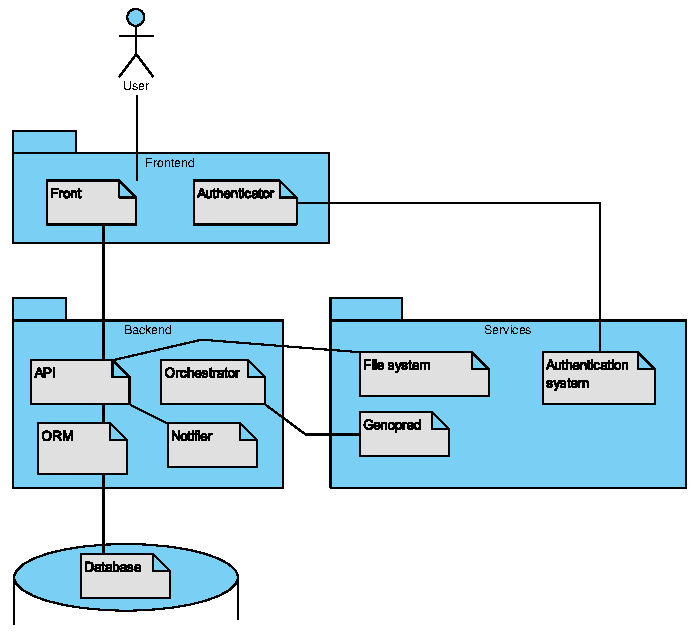
\includegraphics[width=0.9\textwidth]{tfgetsinf/images/high level diagram_cropped.pdf}
    \caption{Diagrama de Alto Nivel}
    \label{fig:highlevel}
\end{figure}


\subsection{Diagrama de componentes}

La representación de componentes de la Figura~\ref{fig:componentes} muestra la estructura de software de \textit{Phenoscore}, desagregada en sus distintos módulos principales y su relación con los servicios externos. Este enfoque modular permite separar responsabilidades y facilita el mantenimiento y la escalabilidad del sistema. A continuación, se detallan los componentes de acuerdo a su dominio de actuación, especificando las tecnologías utilizadas:

\begin{enumerate}
    \item \textbf{Aplicación Principal (\textit{Phenoscore})}
    Es el corazón del sistema, construido como una aplicación \textit{full-stack} unificada con el \textit{framework} \textit{Next.js}. En él se contienen tanto los módulos de la interfaz de usuario (\texttt{frontend}) como los de la lógica de negocio (\texttt{backend}).
    \begin{itemize}
        \item \textbf{Frontend}:
        
            \begin{itemize}
                \item \textbf{Interfaz de Usuario (\textit{Next.js/React}):} Se trata del componente que lleva a cabo la representación de la interfaz web con la que el usuario final interactúa. Implementado en \textit{React}, ofrece los formularios de configuración, muestra el seguimiento de los análisis y la visualización de los resultados.
                \item \textbf{Authenticator}: Módulo cliente que se encarga de manejar el proceso de \textit{login}. Se comunica directamente con \textit{Auth0}, el proveedor de identidad, para verificar las credenciales del usuario y recibir los tokens de acceso, garantizando que únicamente usuarios legítimos accedan a la aplicación.
            \end{itemize}
            
        \item \textbf{Backend}:
        
            \begin{itemize}
                \item \textbf{API (\textit{Next.js}):} Proporciona los \textit{endpoints} \textit{RESTful} que comunican el \texttt{frontend} con la lógica de negocio. Gestiona las peticiones para crear análisis, consultar su estado y obtener resultados.
                \item \textbf{Orchestrator}: Es el núcleo de la lógica del \texttt{backend}. Administra el flujo de ejecución completo: desde la llegada de una nueva petición de análisis, la validación de los datos, la interacción con el \texttt{File System} para el manejo de archivos, la llamada a \texttt{Genopred} vía \texttt{ChildProcess}, hasta la recogida y el almacenamiento de los resultados en la base de datos con \texttt{Prisma}.
                \item \textbf{Prisma}: Actúa como cliente \textit{ORM (Object-Relational Mapping)} para gestionar la conexión y la comunicación con la base de datos \texttt{MySQL}. Permite consultar, insertar y actualizar los datos de los análisis, modelos y usuarios de una forma segura y tipada.
                \item \textbf{ChildProcess}: Es el módulo de \textit{Node.js} utilizado para ejecutar y gestionar procesos externos. Su función es fundamental para invocar \texttt{Genopred}, permitiendo que el análisis se ejecute de forma asíncrona sin bloquear el servidor principal.
                \item \textbf{Notifier}: El componente que gestiona el envío de notificaciones al usuario (por ejemplo, por correo electrónico) cuando un análisis ha finalizado o ha ocurrido un error.
                \item \textbf{Logger}: Módulo encargado de registrar los eventos relevantes del sistema (ej. inicio de un análisis, errores, finalización) para facilitar el diagnóstico, la auditoría y la trazabilidad de las operaciones.
            \end{itemize}
    \end{itemize}
    \item \textbf{Infraestructura Local}
    Conjunto de componentes que se ejecutan en el mismo entorno físico que la aplicación, pero que no forman parte directa del código base del proyecto.

    \begin{itemize}
        \item \textbf{File System}: Representa el sistema de archivos del servidor. Es utilizado por el \texttt{Orchestrator} para almacenar temporalmente los datos genómicos de los pacientes subidos por el usuario, los modelos PRS seleccionados y los ficheros de resultados generados por \texttt{Genopred}.
        \item \textbf{Genopred}: Es el motor de cálculo bioinformático. Se trata de una herramienta externa especializada en ejecutar los análisis de Puntuación de Riesgo Poligénico. El \texttt{Orchestrator} lo invoca como un proceso externo para realizar los cálculos computacionalmente pesados.
    \end{itemize}

    \item \textbf{Servicios de Terceros (\textit{3rd Party Services})}
    Servicios externos con los que el sistema se comunica a través de APIs para delegar funcionalidades específicas.
    \begin{itemize}
        \item \textbf{\textit{Auth0}:} Es el servicio externo de identidad y autenticación. Administra el inicio de sesión y la gestión de los usuarios. El componente \texttt{Authenticator} de la aplicación se conecta a \textit{Auth0} para garantizar un control de acceso robusto y seguro.
        \item \textbf{MySQL Database}: Es el sistema de gestión de base de datos relacional externo donde se persiste toda la información crítica del sistema. El componente \texttt{Prisma} se conecta a esta base de datos para guardar y recuperar datos sobre los análisis, sus configuraciones, estados, resultados y los modelos utilizados.
    \end{itemize}

\end{enumerate}

\begin{figure}[H]
    \centering
    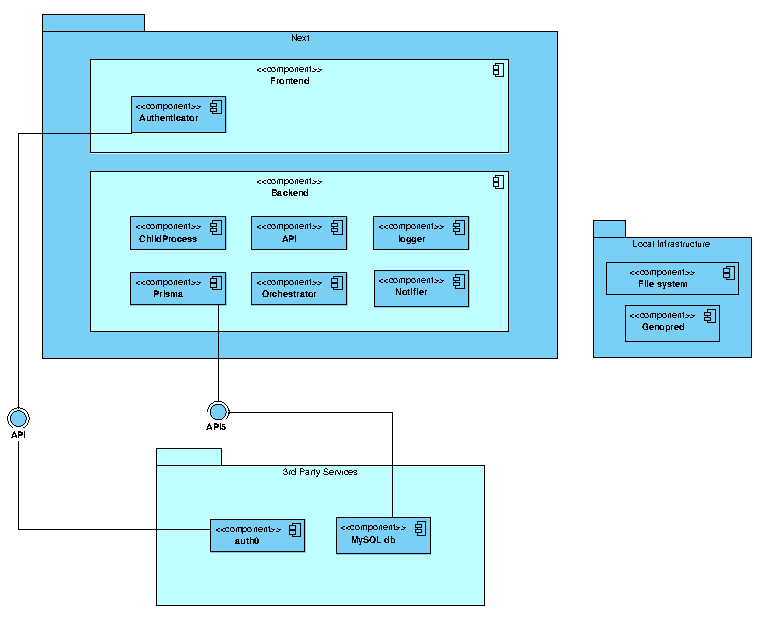
\includegraphics[width=1\textwidth]{tfgetsinf/images/Component Diagram.pdf}
    \caption{Diagrama de Componentes}
    \label{fig:componentes}
\end{figure}


\subsection{Diagramas de secuencia}
Cada diagrama de secuencia representa un flujo clave de funcionalidad, detallando la coreografía de mensajes entre las distintas partes del sistema para alcanzar un objetivo específico. 
Se han consolidado satisfactoriamente las historias de usuario en tres diagramas principales que cubren las funcionalidades más críticas y complejas, y cada uno detalla la coreografía de mensajes entre los distintos componentes.

Los actores y componentes principales del sistema que interactúan en los diagramas de secuencia son los mismos que han sido detalladamente descritos en la sección de Diagrama de Alto Nivel, donde se estableció su rol y responsabilidades dentro de la arquitectura de la plataforma.

\paragraph{Diagrama de secuencia: Inicio de Sesión (\textit{Log In})}
La Figura~\ref{fig:login} detalla el flujo de inicio de sesión de un usuario y la posterior recuperación de sus análisis guardados.

\begin{table}[H]
    \centering
    \small
    \begin{tabular}{|p{6cm}|p{8cm}|}
        \hline
        \textbf{Historias de Usuario Cubiertas} & HU01 (Inicio de sesión) y parcialmente HU02 (Panel de control). \\
        \textbf{Contexto y Precondiciones} & El usuario desea acceder a la aplicación y ya posee una cuenta registrada y válida en el sistema de autenticación externo (\textit{Auth0}). \\
        \hline
    \end{tabular}
\end{table}

El flujo comienza cuando el usuario introduce sus credenciales en el \texttt{Frontend}. Este envía la solicitud a la API, que a su vez la delega en el servicio de autenticación externo. Tras una validación exitosa, el servicio devuelve un token de autenticación a la API, que lo reenvía al \texttt{Frontend}. Con el usuario ya autenticado, el \texttt{Frontend} solicita la lista de análisis personales. La API valida de nuevo el token y, a través de \texttt{Prisma}, consulta la base de datos para obtener los análisis del usuario. Finalmente, los datos son devueltos al \texttt{Frontend}, que los muestra en el panel de control.

\begin{figure}[H]
    \centering
    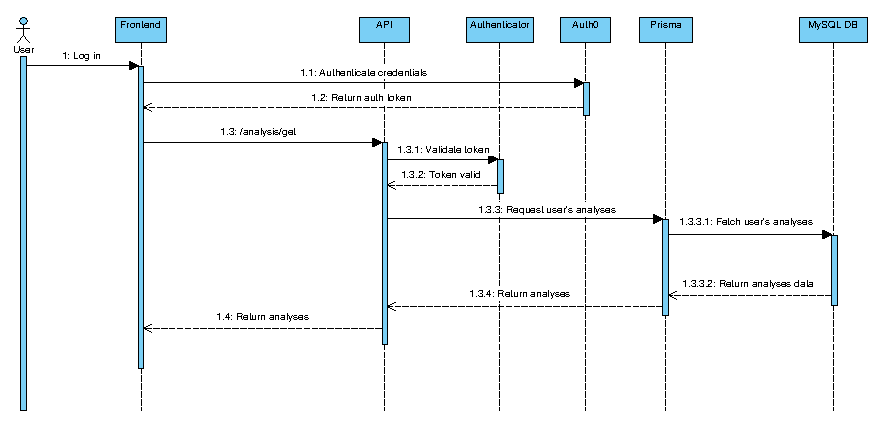
\includegraphics[angle=270, width=0.7\textwidth]{tfgetsinf/images/sequence log in.pdf}
    \caption{Diagrama de Secuencia - Log In}
    \label{fig:login}
\end{figure}

\paragraph{Diagrama de secuencia: Configuración del Análisis}
La Figura~\ref{fig:config} ilustra el proceso de configuración y almacenamiento inicial de los parámetros y archivos de datos para un nuevo análisis PRS.

\begin{table}[H]
    \centering
    \small
    \begin{tabular}{|p{6cm}|p{8cm}|}
        \hline
        \textbf{Historias de Usuario Cubiertas} & HU03 (Crear nuevo análisis), HU05 (Subida de archivos), HU06 (Selección de modelos) y HU07 (Configuración). \\
        \textbf{Contexto y Precondiciones} & El usuario ha iniciado sesión y ha completado el formulario de configuración de un nuevo análisis en la interfaz. \\
        \hline
    \end{tabular}
\end{table}

El proceso se inicia cuando el usuario, tras rellenar el formulario, pulsa el botón para ejecutar el análisis en el \texttt{Frontend}. Este envía una petición \texttt{POST} a la API con toda la configuración. La API interactúa primero con el \texttt{FileSystem Handler} para gestionar y almacenar los ficheros genómicos subidos. Una vez confirmado el almacenamiento de los archivos, la API envía a \texttt{Prisma} la solicitud de guardar todos los parámetros de configuración del análisis en la base de datos. Cuando \texttt{Prisma} confirma que los datos han sido persistidos, la API notifica al \texttt{Frontend} que la configuración se ha guardado con éxito, dejando todo listo para la fase de ejecución.

\begin{figure}[H]
    \centering
    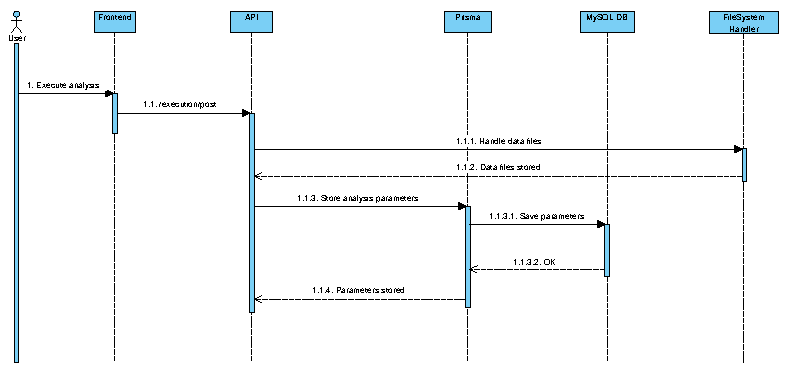
\includegraphics[angle=270, width=0.7\textwidth]{tfgetsinf/images/sequence configuration.pdf}
    \caption{Diagrama de Secuencia - Configuración del Análisis}
    \label{fig:config}
\end{figure}

\paragraph{Diagrama de secuencia: Ejecución del Análisis}
La Figura~\ref{fig:exec} describe el flujo asíncrono de la ejecución de un análisis PRS, desde que se inicia hasta que se notifica el resultado al usuario.

\begin{table}[H]
    \centering
    \small
    \begin{tabular}{|p{6cm}|p{8cm}|}
        \hline
        \textbf{Historias de Usuario Cubiertas} & HU08 (Ejecución del análisis) y HU11 (Notificaciones). \\
        \textbf{Contexto y Precondiciones} & El análisis ha sido configurado y sus parámetros están almacenados en la base de datos. \\
        \hline
    \end{tabular}
\end{table}

Este flujo, típicamente disparado por un evento interno, comienza cuando la API envía una orden al \texttt{Orchestrator} para iniciar un análisis. El \texttt{Orchestrator} recupera los datos y delega la ejecución del cálculo bioinformático en la herramienta externa \texttt{GenoPred}, proporcionándole todos los parámetros necesarios. Tras un tiempo de procesamiento, \texttt{GenoPred} notifica al \texttt{Orchestrator} que el análisis ha finalizado. A continuación, el \texttt{Orchestrator} envía los resultados (puntuaciones, percentiles) a \texttt{Prisma} para que los guarde en la base de datos. Una vez almacenados, invoca al \texttt{Notifier} para informar al usuario del resultado. Finalmente, la API actualiza el estado del análisis en el \texttt{Frontend}, que muestra al usuario que el proceso ha sido completado.

\begin{figure}[H]
    \centering
    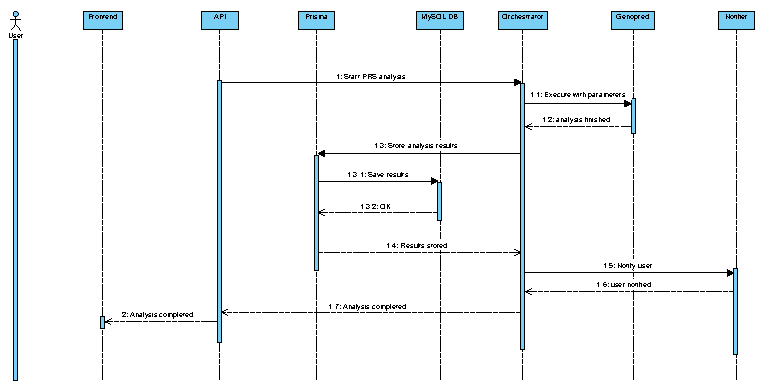
\includegraphics[angle=270, width=0.7\textwidth]{tfgetsinf/images/sequence execution.pdf}
    \caption{Diagrama de Secuencia - Ejecución del Análisis}
    \label{fig:exec}
\end{figure}


\subsection{Arquitectura lógica}

Siguiendo con las decisiones arquitectónicas diseñadas en los modelos mostrados anteriormente, la estructura consta de tres capas diferenciadas que facilitan la separación de responsabilidades \cite{fowler}.

\textbf{Capa de Presentación (\texttt{Frontend}):}
Esta capa es responsable de implementar la interfaz de usuario y de gestionar cualquier interacción directa con el usuario final. Algunas de las funcionalidades clave incluyen la configuración y visualización de análisis PRS, la aplicación de filtros para organizar la información y una presentación interactiva de resultados. El desarrollo utilizó \textit{Next.js} y \textit{React}, dando énfasis a la usabilidad y accesibilidad, lo que llevó a una experiencia de usuario intuitiva y eficiente.

\textbf{Capa de Lógica de Negocio (\texttt{Backend}):} compuesta por una API construida en \textit{Node.js}, esta capa es la responsable de la conexión entre el \texttt{frontend}, la base de datos y la herramienta \texttt{Genopred}. Entre las funcionalidades más destacables se encuentran la coordinación de la ejecución de los análisis, incluyendo la invocación de procesos externos (\textit{child-process}) para integrar \texttt{Genopred} y la lógica de peticiones.

\textbf{Capa de Datos:} se gestiona mediante una base de datos en \texttt{MariaDB}, a la que se accede y manipula a través del \textit{ORM} \texttt{Prisma}. En esta capa se almacena toda la información persistente del sistema, como los análisis vinculados al usuario, los modelos PRS disponibles, los resultados generados por cada análisis, etc.


\subsubsection{Capa de presentación (\texttt{frontend})}
Esta capa es responsable de la interfaz de usuario. Para su implementación se ha seleccionado \textit{Next.js}, un \textit{framework} basado en \textit{React}. Esta elección permite crear una aplicación web rápida y eficiente mediante el renderizado en el servidor (\textit{SSR}) y la generación de sitios estáticos (\textit{SSG}). Para la estilización de los componentes, se utiliza \textit{PostCSS} para aplicar transformaciones avanzadas sobre \textit{CSS}.
%(Aquí sigue el resto de la sección con los mockups y su conexión a los requisitos, como te mostré antes...)

\textbf{Interfaz gráfica}

Como paso previo a la implementación de las interfaces, se han diseñado los prototipos (o \textit{mockups}) que se emplean para mostrar la idea inicial del funcionamiento de la \textit{app} que posteriormente se va a desarrollar. Se ha hecho uso de la herramienta \textit{Figma}, una herramienta web dedicada a los diseños gráficos y de interfaces. Además, concede la opción de compartir estos prototipos; es una funcionalidad que resulta muy atractiva pensando en la validación de los \textit{mockups} por parte de los usuarios.

Cada pantalla está diseñada para dar respuesta a una o varias de las historias de usuario definidas en la sección de requisitos, asegurando que el diseño esté directamente alineado con las necesidades de los usuarios. A continuación, se presentan los prototipos de las pantallas principales.

\noindent La interfaz se divide en las siguientes pantallas:

\vspace{0.8em}
\noindent\textbf{\textit{Pantalla: Inicio de sesión}}
\vspace{0.8em}

Esta pantalla es la puerta de acceso a la plataforma de forma segura. Inicialmente, el diseño contemplaba la implementación de un formulario de inicio de sesión propio; no obstante, por motivos de seguridad y para simplificar la compleja gestión de identidades, se ha optado por confiar en un servicio externo como \textit{Auth0}. Por tanto, el diseño final (Figura~\ref{fig:mockup-login}) se centra en un simple botón que redirige al usuario a iniciar su flujo de autenticación con un proveedor externo.

 Este diseño cubre directamente la necesidad de \textit{HU01: Inicio de sesión}, que requiere que los usuarios puedan acceder de forma segura con sus credenciales para visualizar sus análisis personales.

\begin{figure}[H]
    \centering
    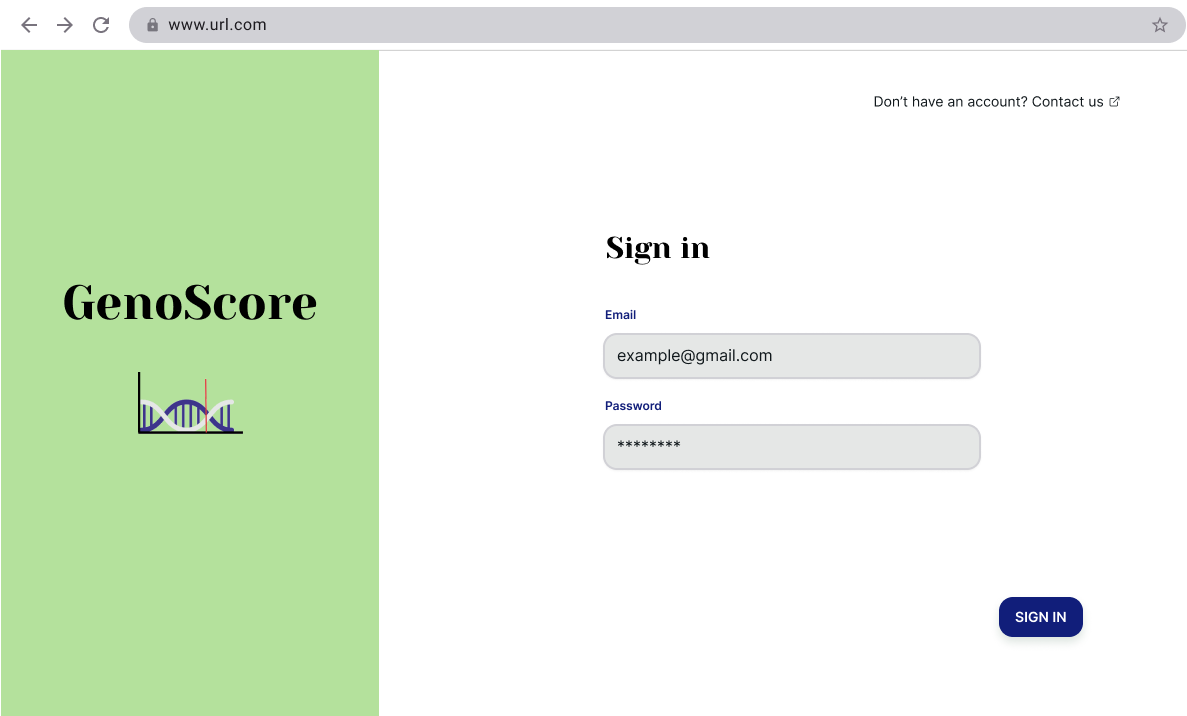
\includegraphics[width=1\textwidth]{tfgetsinf/images/Log in.png}
    \caption{Mockup de Inicio de sesión}
    \label{fig:mockup-login}
\end{figure}

\vspace{0.8em}
\noindent\textbf{\textit{Pantalla: Análisis PRS}}
\vspace{0.8em}

Esta es la pantalla de inicio o panel de control de la aplicación. El componente central (Figura~\ref{fig:mockup-home}) es una tabla que muestra todos los análisis del usuario, permitiendo buscar, consultar el estado o realizar acciones como consultar los resultados o eliminar. La interfaz dispone además de botones para crear nuevos análisis y para abrir un panel de filtros (Figura~\ref{fig:mockup-filtros}), que permite limitar la vista por paciente, estado o fecha.

Las historias de usuario cubiertas por esta pantalla son: \textit{HU02: Panel de control}, al proporcionar una vista centralizada del estado y progreso de todos los análisis y \textit{HU04: Gestión de análisis PRS}, ya que permite visualizar, ordenar y eliminar los estudios existentes.


\begin{figure}[H]
    \centering
    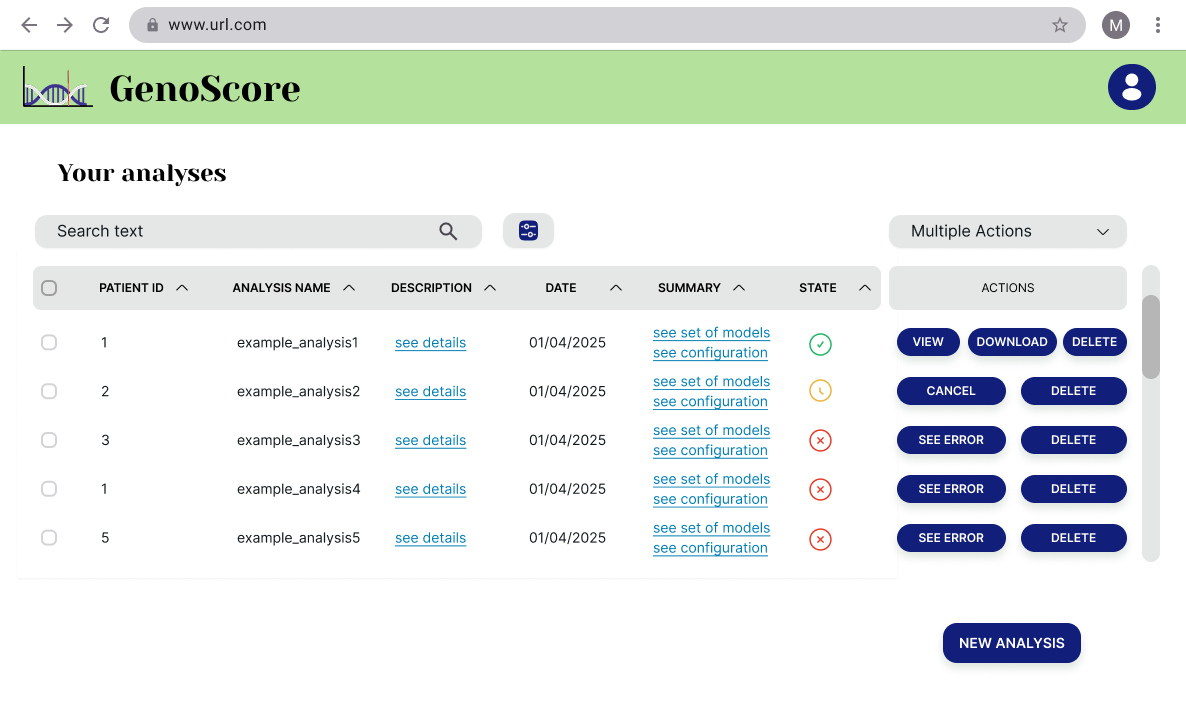
\includegraphics[width=1\textwidth]{tfgetsinf/images/Home.png}
    \caption{Mockup de Análisis PRS}
    \label{fig:mockup-home}
\end{figure}

\vspace{0.8em}
\noindent\textbf{\textit{Pantalla: Filtros}}
\vspace{0.8em}

Para gestionar cómodamente un elevado número de análisis, se ha diseñado un panel lateral de filtros tal y como se muestra en la Figura~\ref{fig:mockup-filtros}. Esta funcionalidad permite al usuario delimitar los resultados que se le muestran en la tabla principal según unos criterios determinados que le interesen, y así hacer de una forma más eficiente sus búsquedas. En el prototipo se incluyen tres tipos de filtros: por identificador de paciente, por estado del análisis (completado, en proceso, error) y por fecha de creación.

A pesar de que no se ha creado una historia de usuario pensando solo en los filtros, la funcionalidad de los mismos es una aplicación directa que da apoyo a la \textit{HU04: Gestión de análisis PRS}. Al facilitar que el usuario ''visualice y ordene estudios como prefiera'', los filtros son una pieza fundamental para realizar esta tarea, sobre todo cuando llegan a haber muchos análisis en el sistema.

\begin{figure}[H]
    \centering
    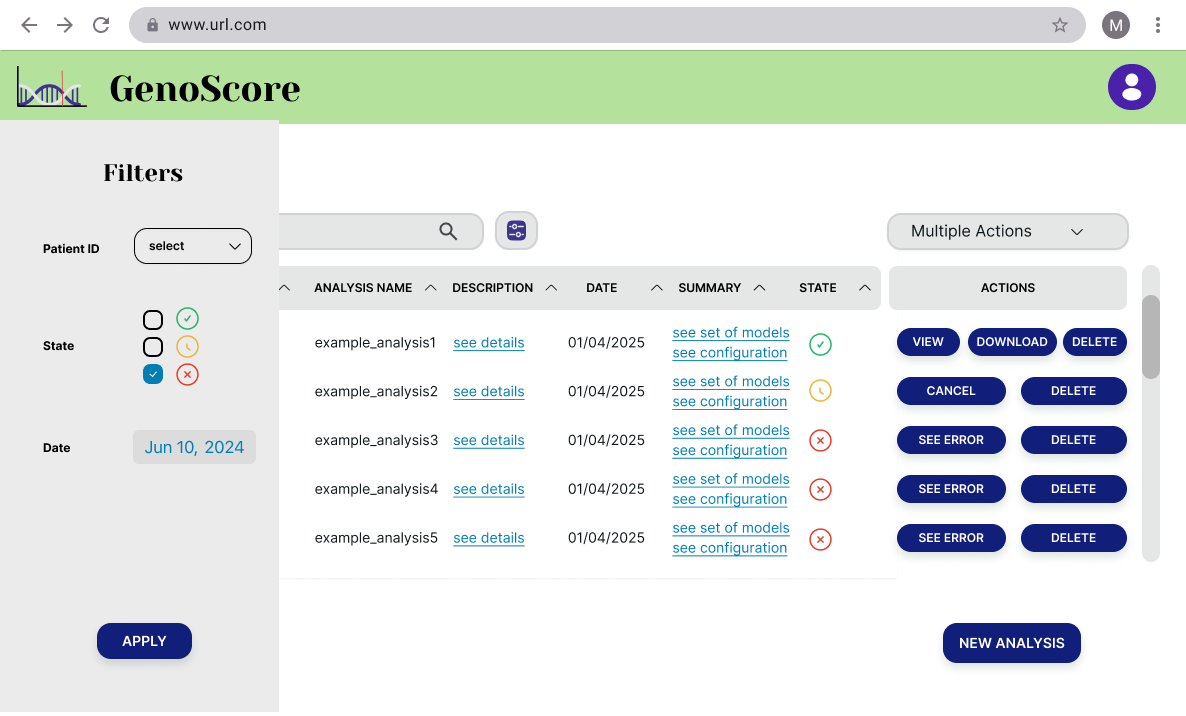
\includegraphics[width=1\textwidth]{tfgetsinf/images/Filtros.png}
    \caption{Mockup de Filtros}
    \label{fig:mockup-filtros}
\end{figure}

\vspace{0.8em}
\noindent\textbf{\textit{Pantalla: Configuración de Análisis PRS}}
\vspace{0.8em}

Con este formulario (Figura~\ref{fig:mockup-configuración}) el usuario puede crear un nuevo análisis PRS. La pantalla está diseñada en pestañas, para facilitar la introducción de metadatos (nombre, paciente), la subida de los ficheros genómicos, la elección de modelos PRS a incluir en el análisis y la configuración de parámetros técnicos del análisis (umbrales de ancestría, ...)

Esta pantalla es clave en el desarrollo de la plataforma, al cubrir un conjunto de historias de usuario esenciales como: \textit{HU03: Crear nuevo análisis PRS}, al ser el punto de partida para una nueva ejecución, \textit{HU05: Subida de archivos genéticos}, proporcionando la interfaz para cargar los ficheros necesarios, \textit{HU06: Selección de modelos PRS}, mediante el botón de selección de modelos y \textit{HU07: Configuración del análisis}, al permitir al usuario personalizar los parámetros técnicos de la configuración del análisis.

\begin{figure}[H]
    \centering
    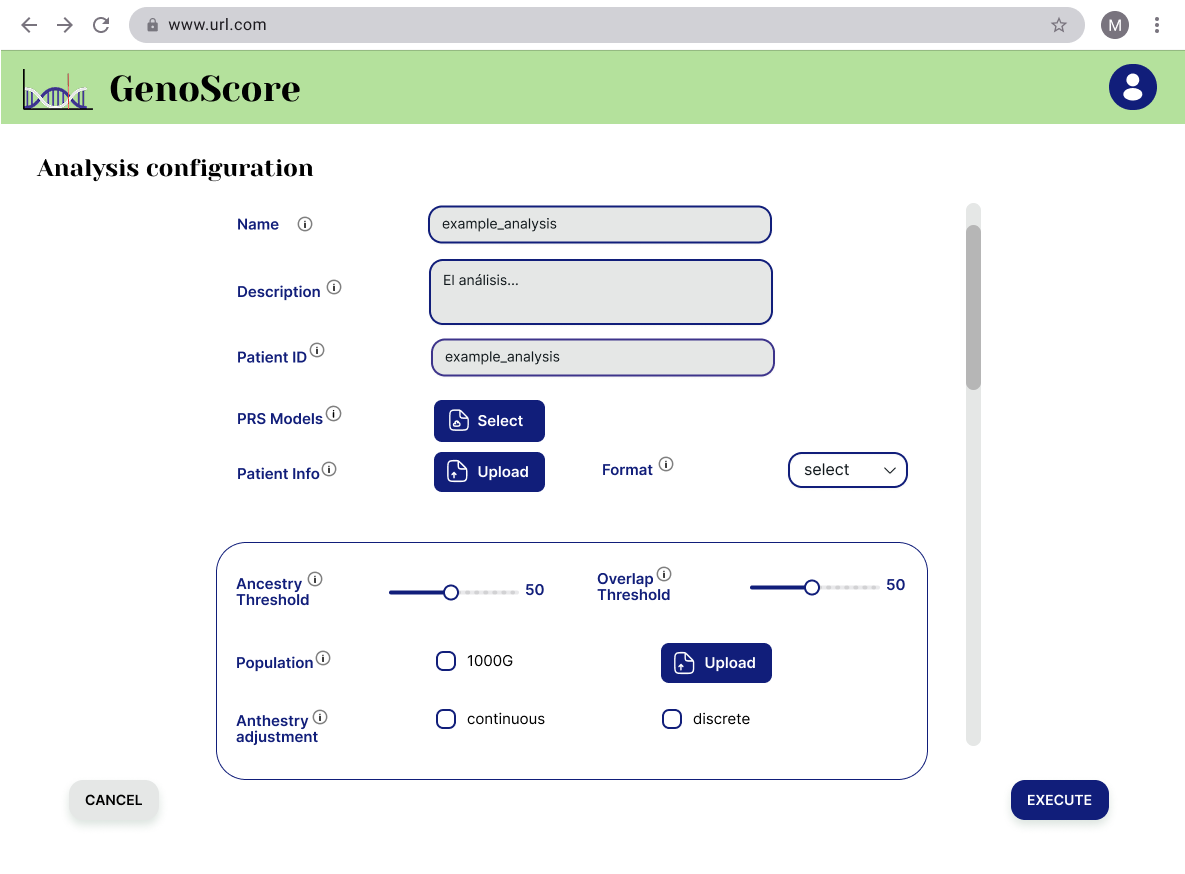
\includegraphics[width=1\textwidth]{tfgetsinf/images/New analysis.png}
    \caption{Mockup de Configuración de Análisis PRS}
    \label{fig:mockup-configuración}
\end{figure}


\subsubsection{Capa de lógica de negocio (\texttt{backend})}
La lógica de negocio se implementa sobre el entorno de ejecución \textit{Node.js}, aprovechando las \textit{API Routes} nativas de \textit{Next.js} para construir los \textit{endpoints} de la API. La comunicación segura y tipada con la base de datos se delega al \textit{ORM} \texttt{Prisma}, que se integra con \textit{TypeScript} para garantizar la corrección de tipos en las consultas.
%(Aquí sigue la descripción del Orquestador, etc...)

\subsubsection{Capa de datos}
Para la persistencia de datos, se ha seleccionado \texttt{MariaDB} como sistema gestor de base de datos relacional. El esquema de la base de datos y las migraciones se gestionan a través de los ficheros de definición de \texttt{Prisma}.
%(Aquí sigue la descripción de la BD con el diagrama E-R y la explicación de las entidades...)
En este apartado se va a detallar el diseño de la arquitectura planteada para el desarrollo de la herramienta propuesta, desde la construcción de la base de datos hasta la interfaz gráfica.

\textbf{Diagrama y estructura de la base de datos}
En la siguiente Figura~\ref{fig:bd}, se puede observar el diagrama de la base de datos; la estructura de este diagrama ha sido acordada junto a otro equipo de investigación, el cual está desarrollando un sistema para la extracción, priorización y aplicación de modelos de puntuación de riesgo poligénico.

La relación con este trabajo es muy relevante, ya que el resultado de priorización de modelos será la lista a seleccionar desde la pantalla de configuración en el campo Models PRS.

En este apartado se ha hecho el paso de un diagrama de clases conceptual (Figura \ref{fig:clases3}) a un diagrama físico de base de datos (Figura \ref{fig:bd}). En el modelo de dominio se modelan aspectos relevantes para describir, entender y comunicar el dominio, pero no se detalla cómo se van a almacenar los datos. Por el contrario, un diagrama de base de datos es un modelo robusto y detallado que indica cómo se tiene que almacenar la información. Este cambio no solo supone cambiar la notación, sino que además supone una ampliación del modelo para dar soporte a las necesidades del sistema.

A continuación, se detallan los cambios más significativos entre ambos diagramas: 

\begin{itemize}
    \item \textbf{Nuevos Atributos en \texttt{PRSAnalysis}:} Se han incluido campos para la gestión de trabajos asíncronos (\texttt{queue\_job\_id}) y notificaciones (\texttt{notification\_email}), que son detalles de implementación que surgen durante el diseño técnico.
    \item \textbf{Nuevas Entidades Añadidas:}
    \begin{itemize}
        \item \texttt{UserNotificationSettings}: Esta tabla almacena las preferencias de notificación personalizadas para cada usuario.
        \item \texttt{UserNotificationHistory}: Esta tabla actúa como un registro o historial de todas las notificaciones enviadas a un usuario.
    \end{itemize}
    \item \textbf{Nueva Relación en \texttt{PRSAnalysis}:}
    La tabla \texttt{PRSAnalysis} ahora está vinculada a estas nuevas entidades. Cuando un análisis finaliza o falla, la aplicación consulta la tabla \texttt{UserNotificationSettings} para determinar cómo notificar al usuario y luego crea una nueva entrada en \texttt{UserNotificationHistory} para registrar el evento.
\end{itemize}

\begin{figure}[H]
    \centering
    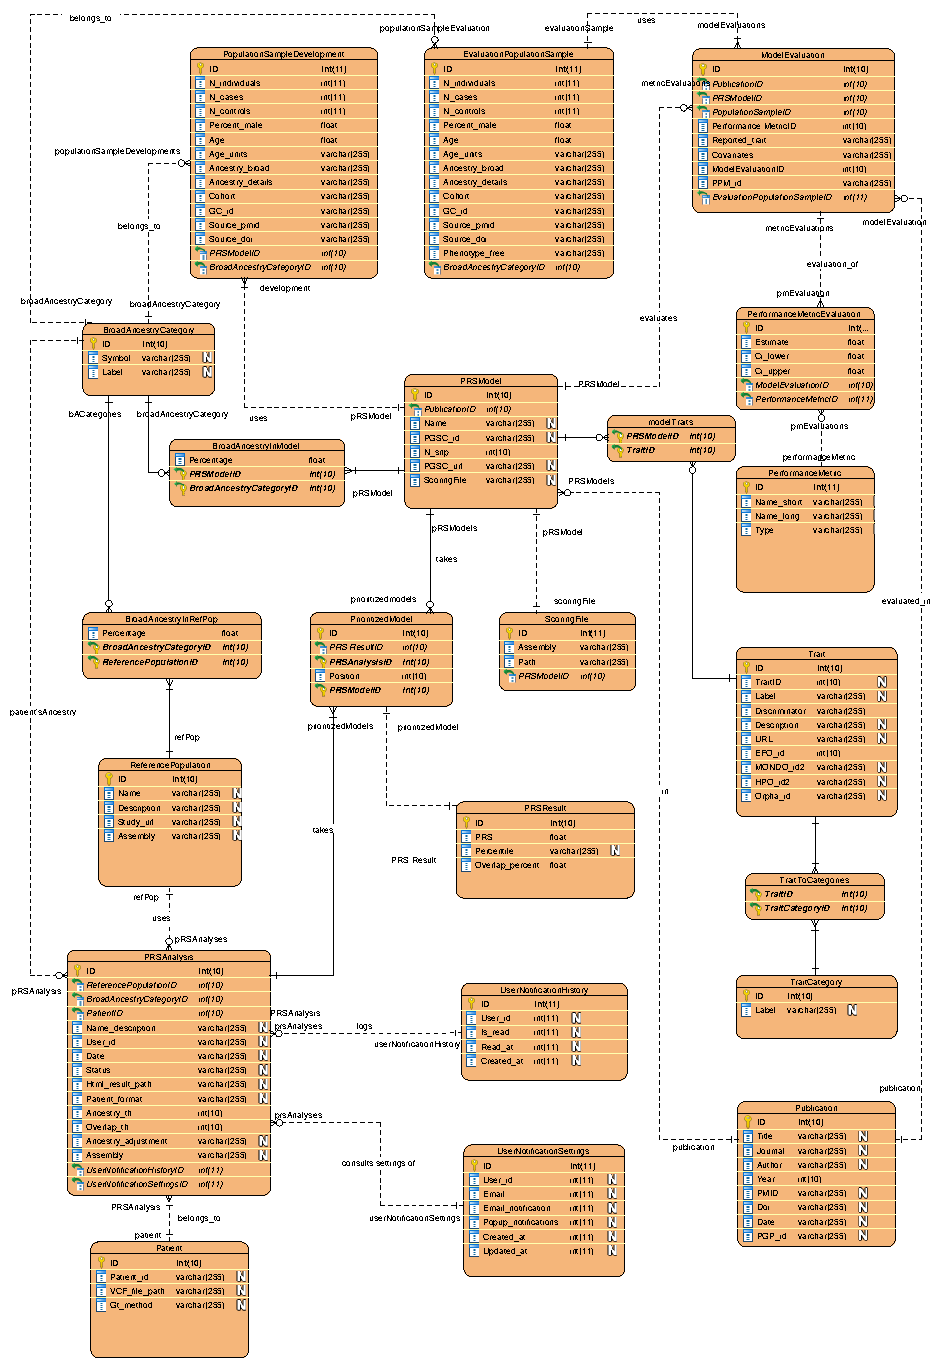
\includegraphics[width=1.1\textwidth]{tfgetsinf/images/ORM Diagram1_cropped (1).pdf}
    \caption{Diagrama de entidad relación}
    \label{fig:bd}
\end{figure}


\subsection{Arquitectura física}

El diseño físico comienza con el diagrama de despliegue representado en la Figura~\ref{fig:despliegue}, que describe la arquitectura del sistema \textit{PhenoScore} en términos de los distintos componentes físicos que lo conforman y cómo está distribuido en una máquina virtual. Un diseño modular como este permite definir mejor qué hace cada componente y poder llevar a cabo un mantenimiento o evolución importante del sistema. 

\begin{figure}[H]
    \centering
    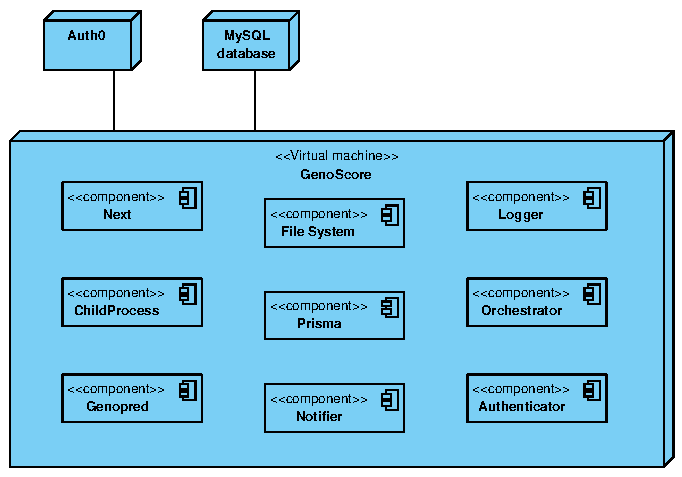
\includegraphics[width=0.9\textwidth]{tfgetsinf/images/Deployment Diagram.pdf}
    \caption{Diagrama de Despliegue}
    \label{fig:despliegue}
\end{figure}

Para el despliegue de la aplicación, se ha optado por un enfoque centralizado en una máquina virtual (VM) dedicada, ubicada en \textit{Google Cloud}. Esta VM ha sido configurada con las siguientes especificaciones: 

\begin{itemize}
    \item Sistema Operativo: \textit{Debian 12 Bookworm}
    \item Tipo de Máquina: e2-standard-2
    \item CPU: 2 CPU virtuales
    \item Memoria RAM: 8 GB
    \item Almacenamiento (Disco de Arranque): 30 GB (Disco persistente balanceado)
\end{itemize}

Esta configuración permite tener un entorno independiente y estable, con el tamaño necesario para sostener las cargas de trabajo tanto de \texttt{frontend} como de \texttt{backend}, así como las pesadas operaciones de cálculo de análisis genético llevadas a cabo por \texttt{Genopred} y la gestión de archivos.

En cuanto a la comunicación con el exterior, la máquina virtual se comunica con los servicios esenciales para su correcto funcionamiento. En primer lugar, mantiene una vía abierta con \textit{Auth0}, el proveedor de identidad, servicio de autorización y gestión segura de accesos, evitando que la aplicación tenga que gestionar sus propios usuarios. Asimismo, establece conexión con la base de datos situada en otro servidor para guardar la información. Se puede consultar en esta arquitectura del sistema las especificaciones funcionales y tecnológicas de los componentes que se encuentran dentro de esta VM (\texttt{Next}, \texttt{Orchestrator}, \texttt{Genopred}, \texttt{Prisma}, etc.).

\section{Desarrollo de la propuesta}
\label{section:desarrollo}

Una vez definidos los requisitos y el diseño de la aplicación, este capítulo se centra en el proceso de implementación de la solución propuesta.
Partiendo del diseño arquitectónico por capas, se detalla la construcción de cada uno de los componentes del sistema, desde la persistencia de los datos hasta la interfaz gráfica.

Asimismo, se exponen los desafíos técnicos encontrados durante el desarrollo y las decisiones tomadas para resolverlos, ofreciendo una visión completa del proceso de ejecución del proyecto y del resultado final obtenido.

\subsection{Herramientas y metodología de desarrollo}
\label{subsec:metodologia_desarrollo}
Para garantizar la calidad, mantenibilidad y eficiencia durante la fase de implementación, se ha seguido una metodología de desarrollo estructurada y se ha hecho uso de un conjunto de herramientas estándar en la industria.

\subsubsection{Entorno y control de versiones}
El entorno de desarrollo principal ha sido \textit{Visual Studio Code (VSC)}, un editor de código ligero y extensible. Por otro lado, el control de versiones del código fuente se ha gestionado utilizando \textit{Git}, manteniendo un historial de cambios en un repositorio de \textit{GitHub}. Esta práctica ha facilitado la colaboración, la trazabilidad y la posibilidad de revertir cambios si fuera necesario.

\subsubsection{Estructura del proyecto}
El código fuente se ha organizado siguiendo un enfoque modular para facilitar su mantenimiento y crecimiento. La estructura principal de directorios es la siguiente:
\begin{itemize}
\item \textbf{/prisma/}: Contiene el esquema de la base de datos definido para \texttt{Prisma} y los ficheros de migración generados automáticamente.
\item \textbf{/public/}: Almacena todos los archivos estáticos que se usan públicamente, como imágenes y fuentes.
\item \textbf{/src/app/}: Es el directorio principal del código fuente de la aplicación \textit{Next.js}, donde se encuentran las páginas, las rutas de la API, los componentes reutilizables (\texttt{/components}), los \textit{hooks} de \textit{React} (\texttt{/hooks})).
\item \textbf{/utils/}: Contiene funciones auxiliares y utilidades compartidas a lo largo de todo el proyecto.
\item \textbf{/services/}: Contiene diferentes servicios como el \textit{worker} de \textit{BullMQ} responsable de ejecutar los análisis de PRS de forma desacoplada, el procesador principal de los análisis junto con el gestor de colas de trabajo y las notificaciones a través del correo electrónico.
\end{itemize}

\subsubsection{Control y calidad de código}
Para mantener un estilo de código consistente y detectar errores de forma temprana, se ha configurado \textit{ESLint}. Este \textit{linter} analiza el código estáticamente, asegurando el cumplimiento de las reglas de estilo y mejorando la legibilidad. Para la estilización, se ha utilizado \textit{PostCSS} para mejorar los estilos \textit{CSS} mediante \textit{plugins} modernos.

\subsubsection{Gestión de dependencias}
El proyecto gestiona sus librerías y dependencias a través del gestor de paquetes \textit{npm}. El fichero \texttt{package.json} actúa como manifiesto, listando todas las dependencias y los scripts necesarios para ejecutar y construir la aplicación.

\subsection{Implementación de la capa de presentación (\texttt{frontend})}
\label{subsec:desarrollo_frontend}
Esta capa es la responsable de la interfaz de usuario y la interacción directa con el usuario final. En este apartado se aborda la evolución de los componentes visuales desde los \textit{mockups} de \textit{Figma} hasta la interfaz final, justificando las decisiones de mejora tomadas durante la implementación. Para acelerar el desarrollo y garantizar una estética moderna y consistente, se ha utilizado la biblioteca de componentes \textit{HeroUI}.

\subsubsection{Inicio de sesión}
En la pantalla de inicio de sesión, a diferencia del \textit{mockup} inicial, que se componía de un formulario de \textit{login} propio, en la versión final se ha integrado \textit{Auth0}, por lo que la implementación específica ha sido a través de este. Esta modificación, como ha sido explicada anteriormente, delega la gestión de usuarios y contraseñas, lo cual fortalece la seguridad del sistema.

Del mismo modo, la barra de navegación que aparece tras el inicio de sesión se ha refinado para mejorar la usabilidad y la accesibilidad. Partiendo de una estructura básica en los \textit{mockups}, la implementación final introduce una organización más funcional. Se han añadido botones de navegación explícitos para las secciones principales y un nuevo control para la gestión de notificaciones. Este último componente, añadido tras considerar el flujo de usuario en procesos largos, permite solicitar avisos por correo sobre la finalización de los análisis, mejorando considerablemente la experiencia de usuario.

\begin{figure}[H]
    \centering
    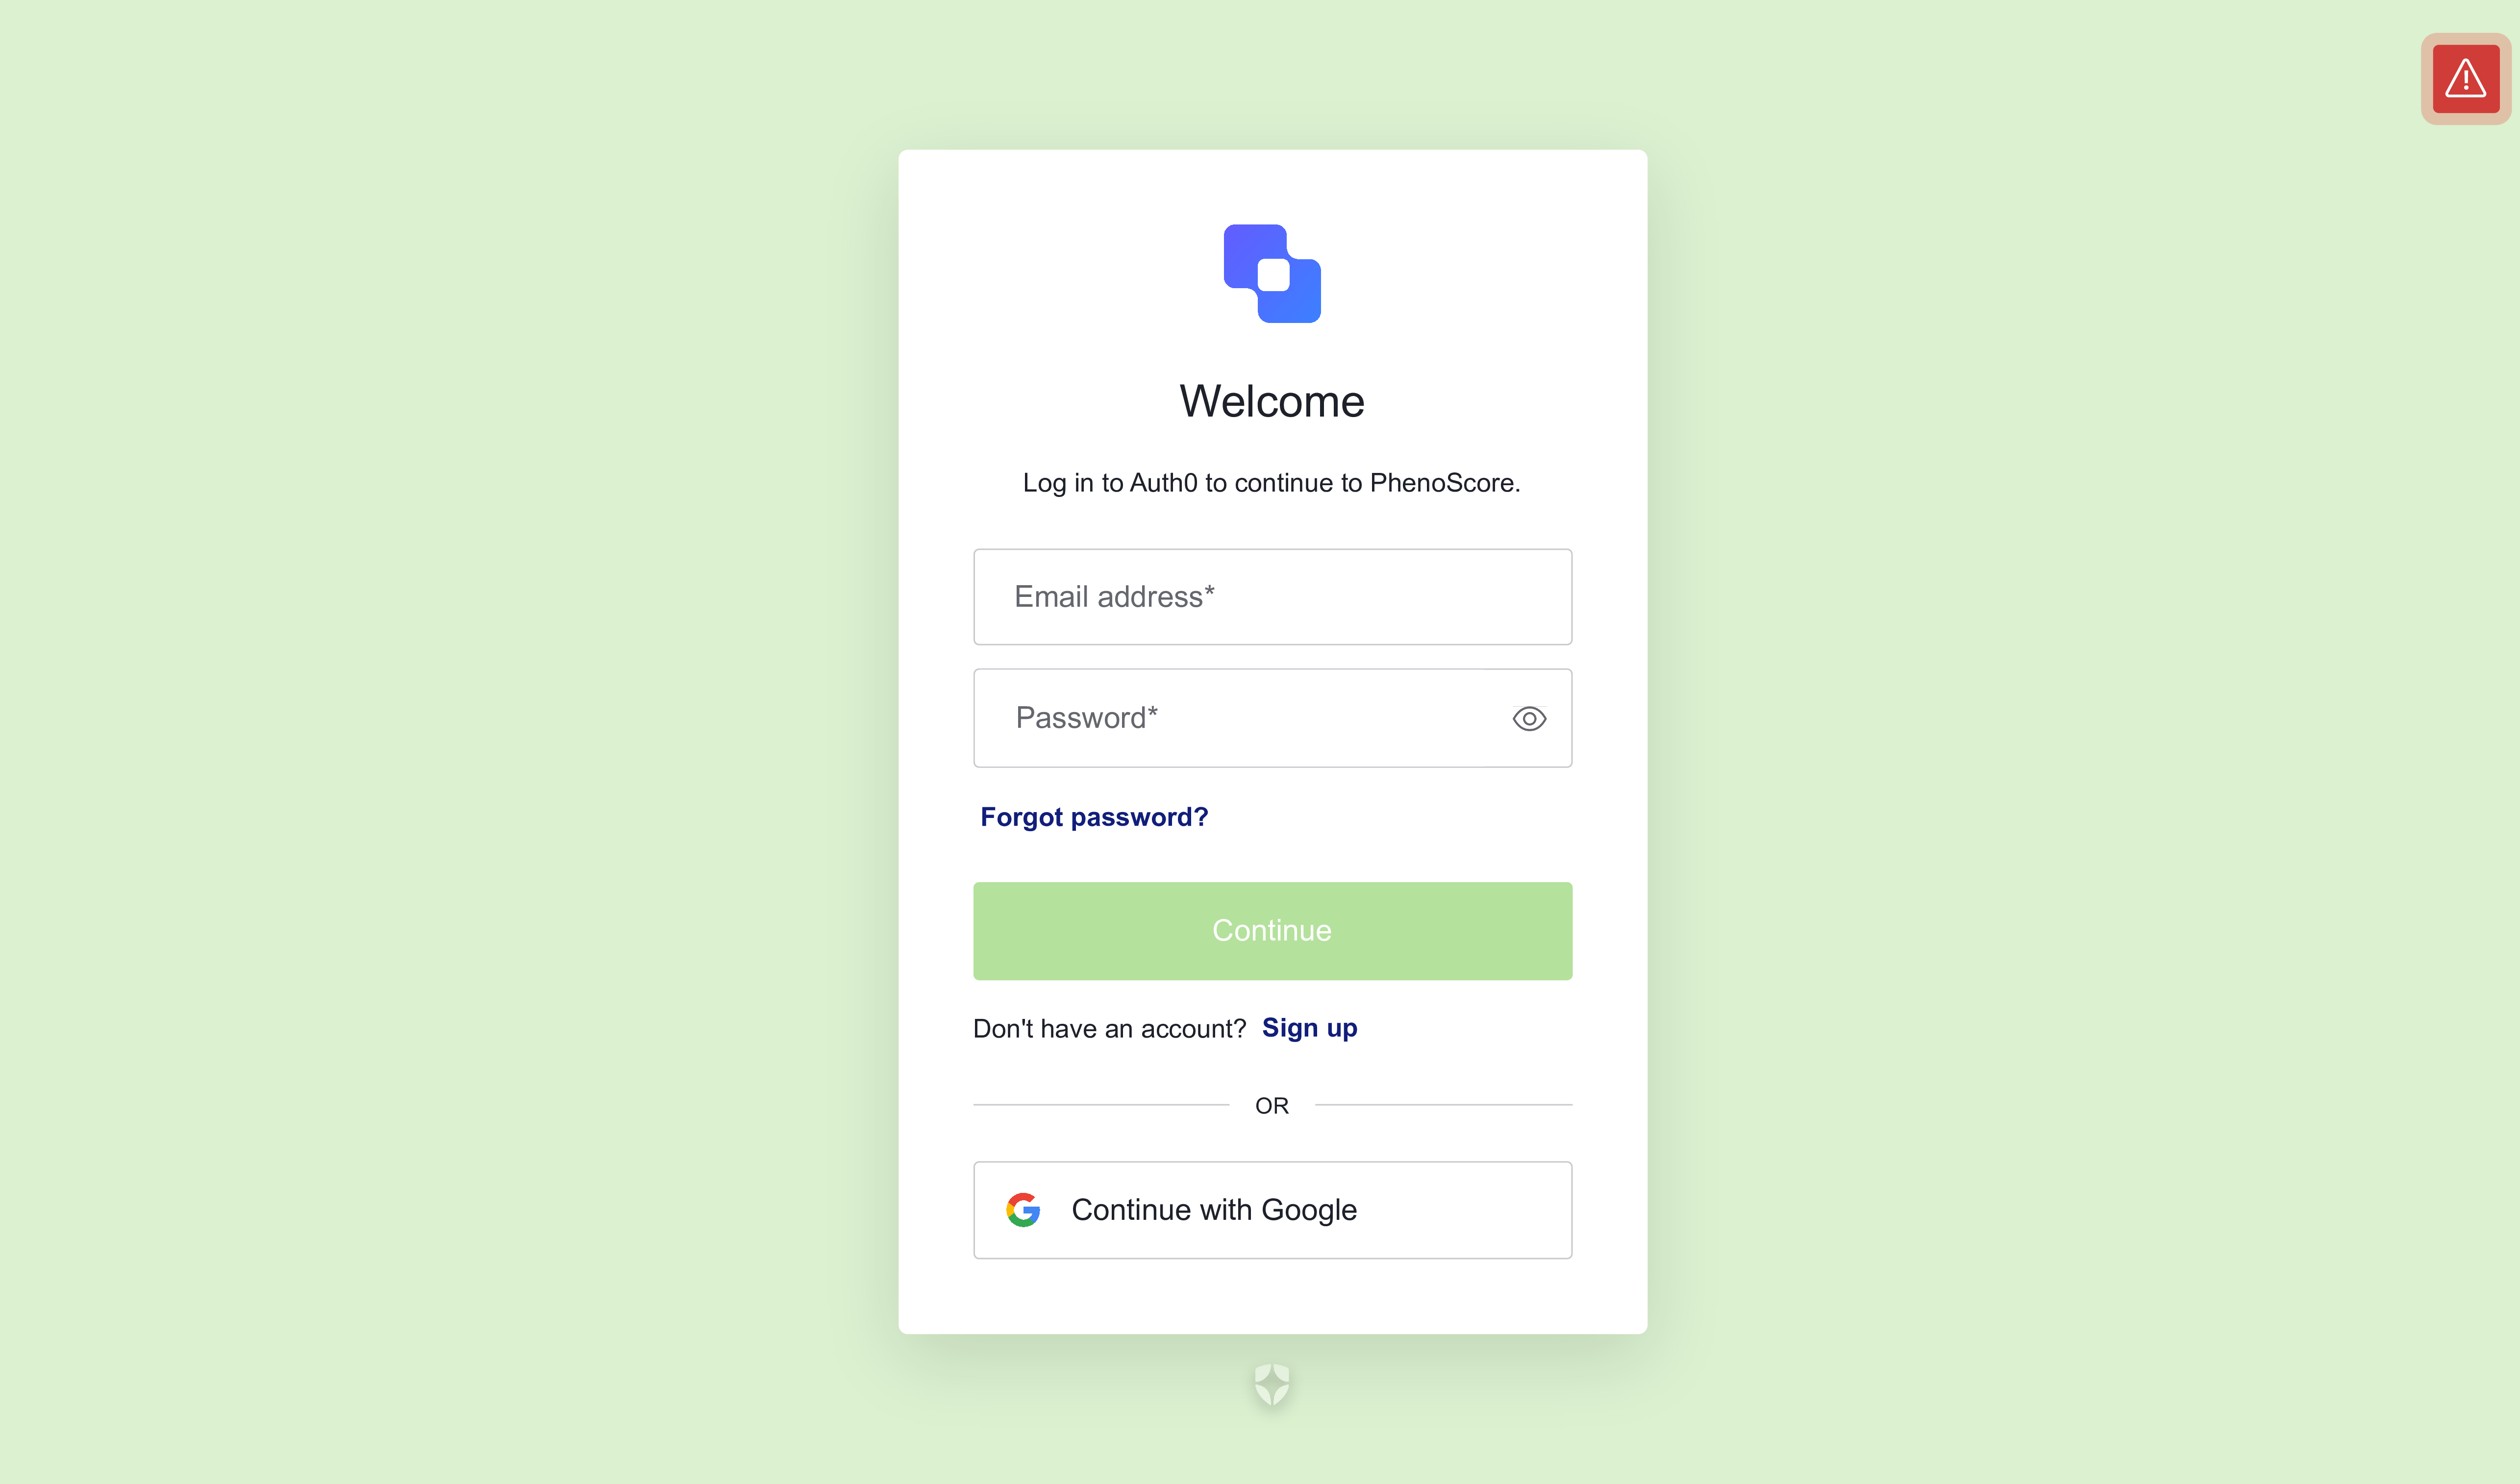
\includegraphics[width=1\textwidth]{tfgetsinf/images/Log-in-_-PhenoScore.png}
    \caption{UI Inicio de sesión}
    \label{fig:UIlogIn}
\end{figure}

\subsubsection{Visualización de análisis PRS}
La implementación de la pantalla de visualización de análisis se ha centrado en optimizar la interacción del usuario y la gestión de la información, materializando las necesidades identificadas en la fase de diseño. Aunque la estructura central sigue siendo la tabla que lista los análisis, se han incorporado varios componentes para mejorar la usabilidad.

El diseño final integra los filtros directamente en la cabecera de la tabla, permitiendo al usuario acotar los resultados de forma rápida y contextual. Adicionalmente, se han implementado controles de visualización que no estaban detallados en los \textit{mockups} iniciales, pero que son esenciales para una experiencia de usuario completa: un selector de columnas para personalizar la información mostrada y un control de paginación para gestionar eficientemente un gran volumen de análisis. Estas funcionalidades, implementadas siguiendo patrones de diseño de interfaces de datos, aseguran que la interacción del usuario con la tabla sea intuitiva y eficiente.

\begin{figure}[H]
    \centering
    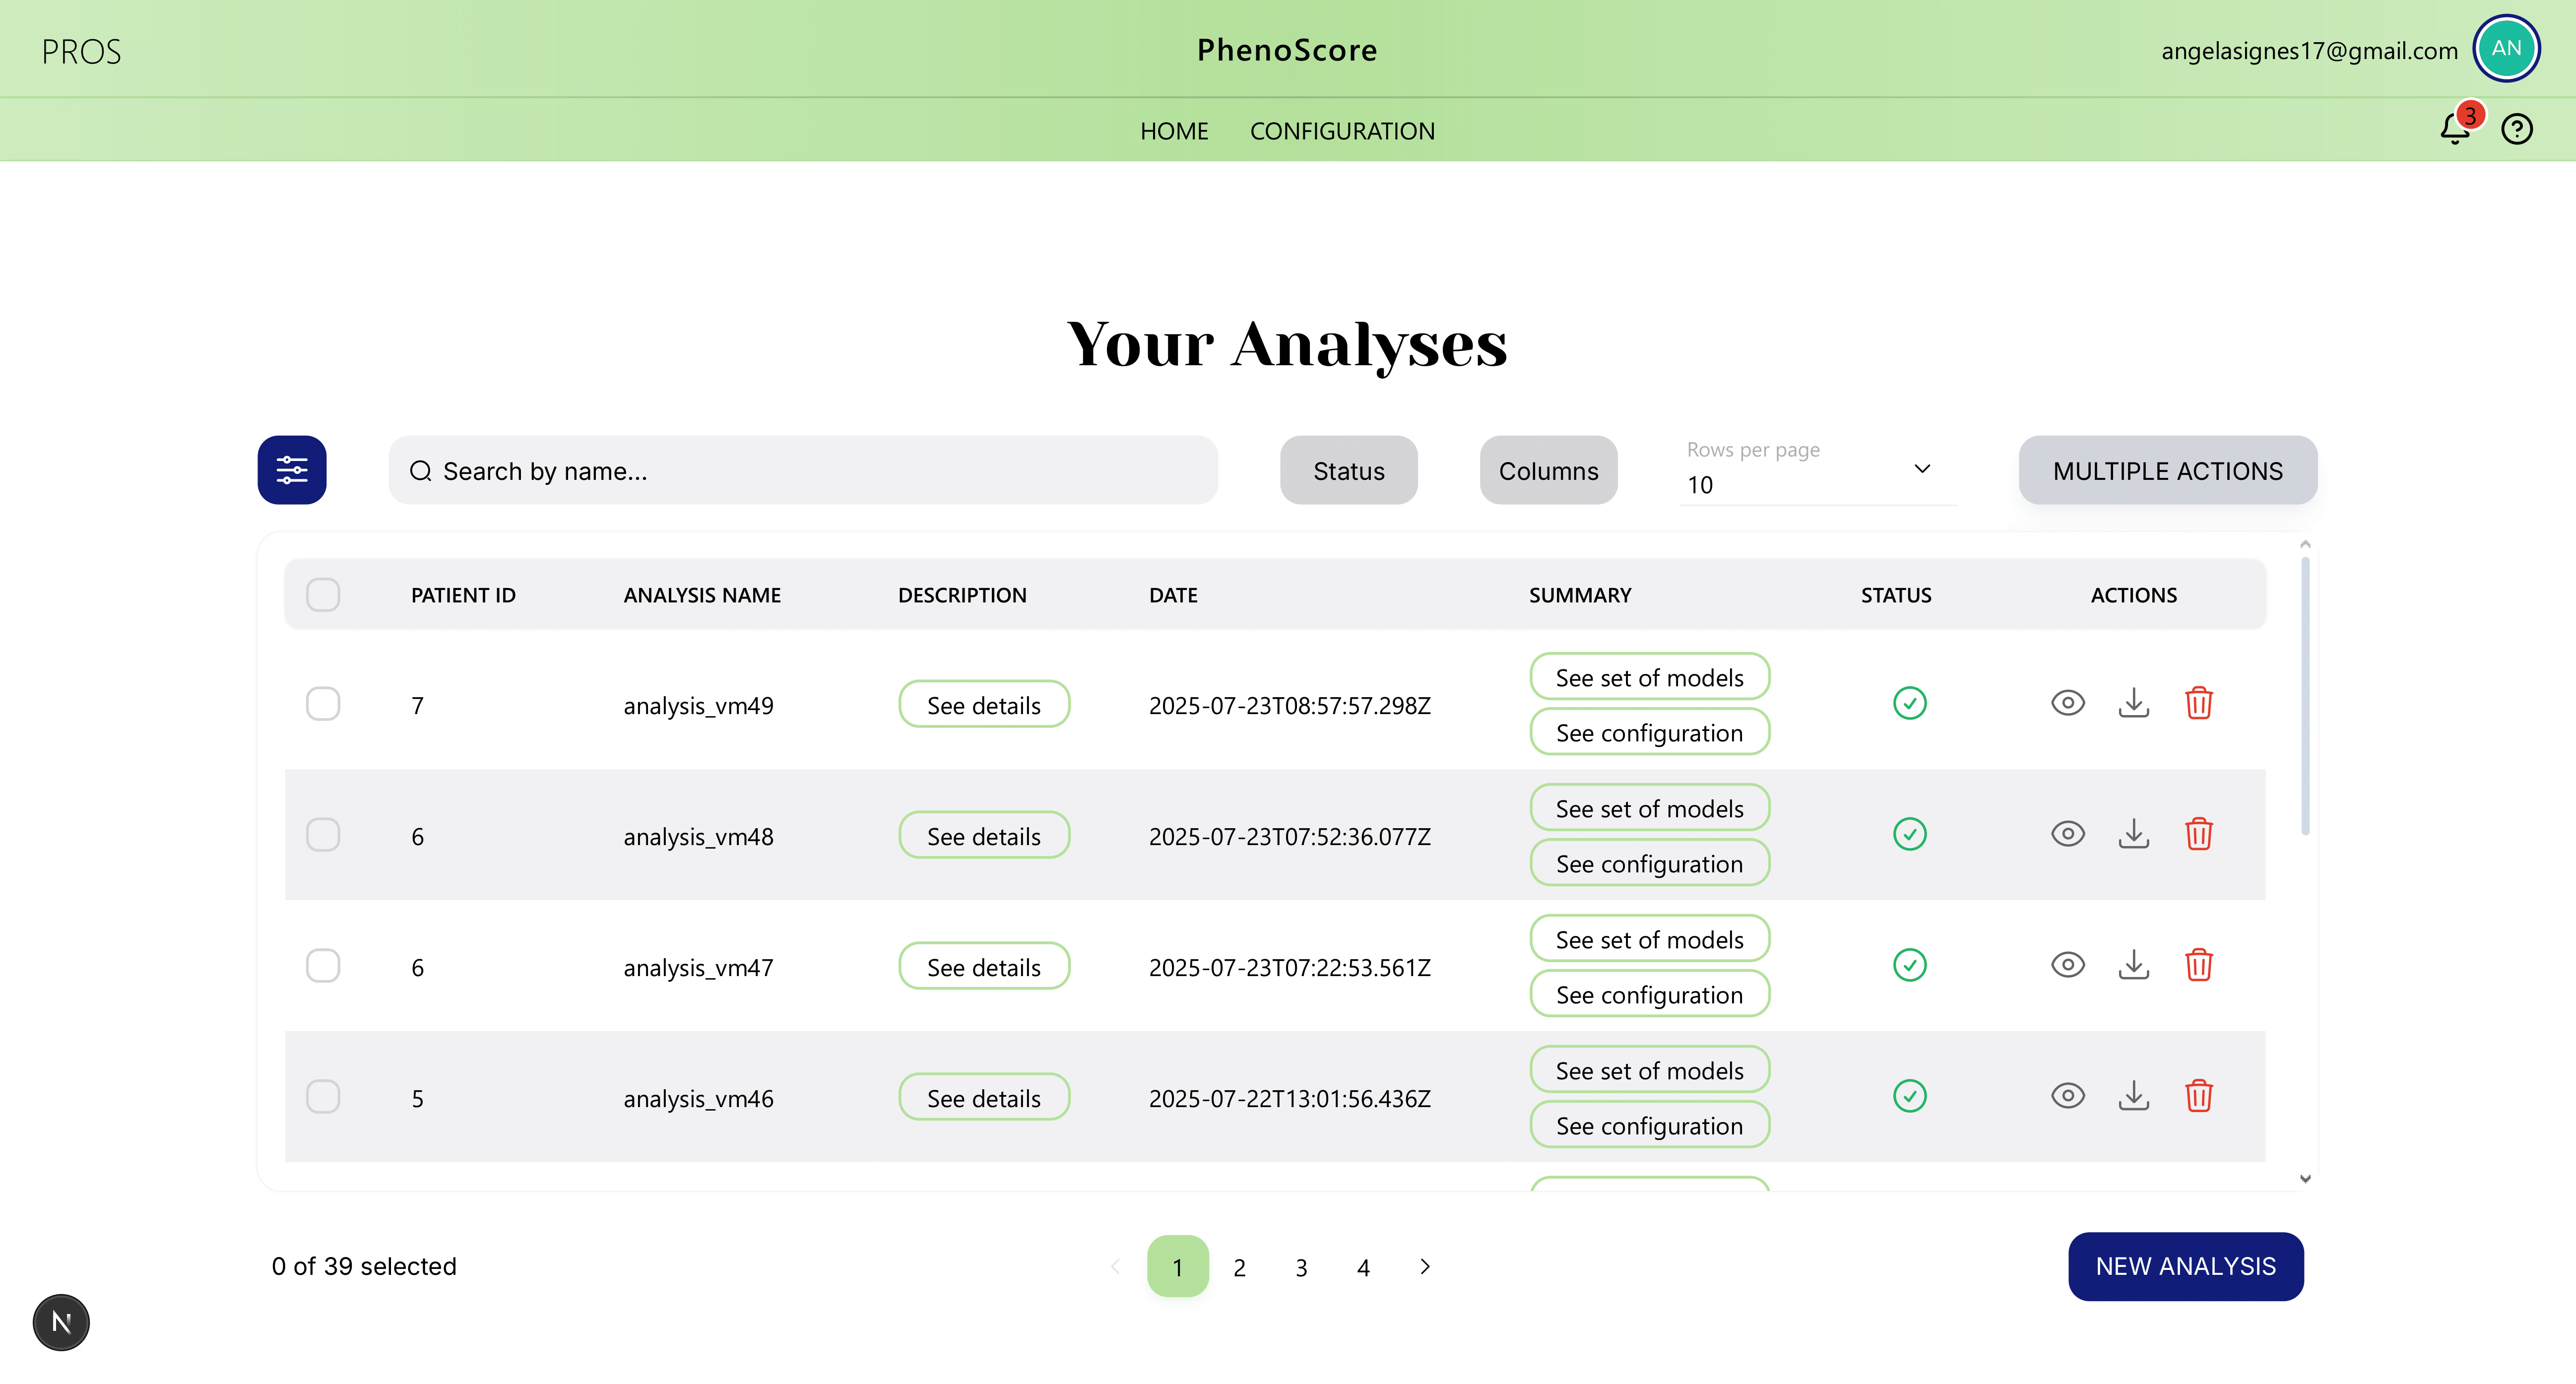
\includegraphics[width=1\textwidth]{tfgetsinf/images/home-1.png}
    \caption{UI Visualización de análisis PRS}
    \label{fig:UIVisualización}
\end{figure}

\subsubsection{Configuración de análisis PRS}
La pantalla de configuración es donde se concentran las modificaciones más relevantes y, además, donde se ha reflejado un cambio de necesidades por parte de los investigadores.

En primer lugar, se dividió el formulario en dos secciones claramente diferenciadas. Por un lado, los datos propios del análisis, como ficheros de entrada o parámetros, y, por otro lado, la configuración detallada de la población de referencia. Se aplicó el principio de separación de responsabilidades para que el proceso de configuración fuera más sencillo para el usuario; de esta forma se minimiza la posibilidad de errores.

En la sección de la población de referencia, se eliminó la opción explícita de ''1000 Genomes Reference'', estableciéndola como opción por defecto a menos que el usuario proporcione una alternativa. Además, se han añadido dos botones que mejoran la recopilación de datos: uno que dirige a una lista para completar la información sobre los detalles de la población de referencia cargada y otro que visualiza la distribución de la ascendencia. Esta última lista ha sido considerada de gran importancia, ya que permite evaluar la categoría de ascendencia en la referencia para una estratificación poblacional precisa.

Finalmente, los botones tradicionales para subir ficheros fueron reemplazados por componentes de arrastrar y soltar. Este cambio, aparte de ser estético, ofrece una experiencia de usuario superior, al ser más interactivos y visuales. El uso de la librería \textit{react-dropzone} ha facilitado la gestión de la carga y la validación de los ficheros.

\begin{figure}[H]
    \centering
    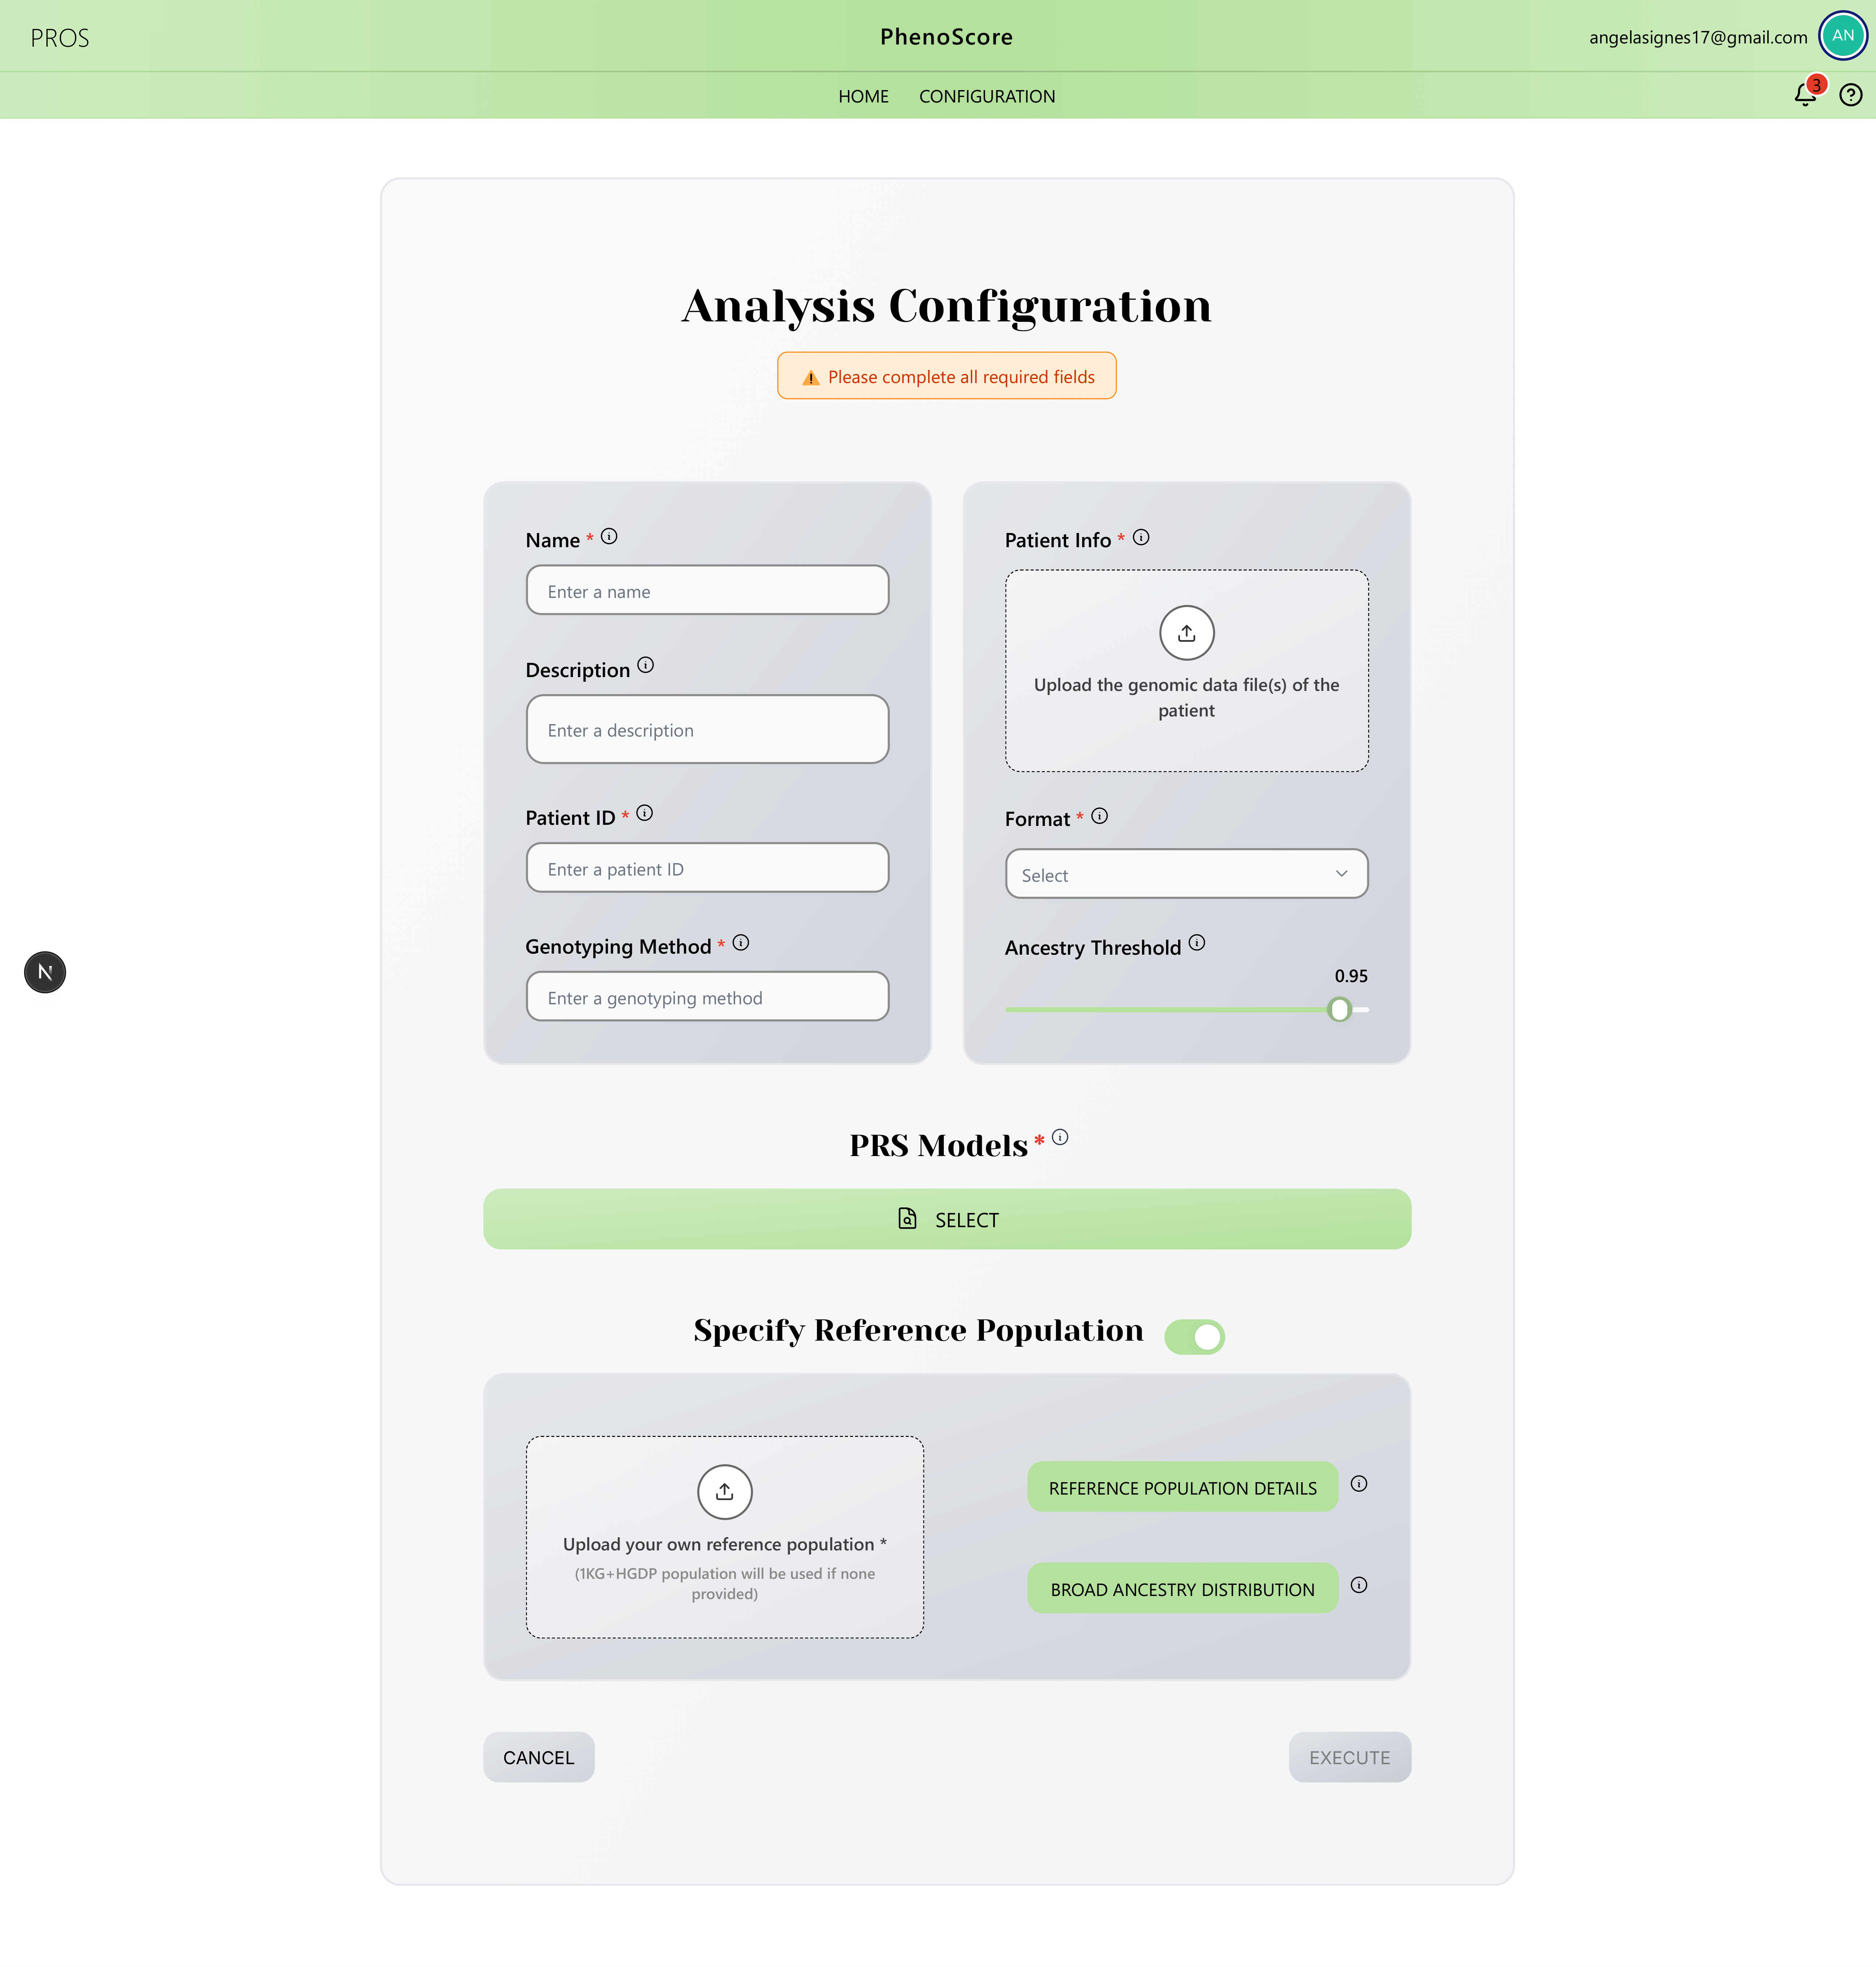
\includegraphics[width=1\textwidth]{tfgetsinf/images/configuration-1.png}
    \caption{UI Configuración de análisis PRS}
    \label{fig:UIConfiguración}
\end{figure}

\subsubsection{Configuración de las notificaciones}
En este modal, abierto desde la configuración del usuario en el perfil, se encuentra la estructura de las opciones de preferencia sobre la funcionalidad de las notificaciones en la \textit{app} y el correo. Además, se ofrece información del usuario de \textit{Auth0} con el que se navega en la \textit{app} y el email ligado a la cuenta.

Este sistema se basa en mantener a los usuarios informados del estado de sus análisis PRS. Acerca de las notificaciones en la \textit{app}, se implementa un historial con los últimos avisos que no hayan sido descartados anteriormente. Por otro lado, la lógica por correo ha hecho uso de diversos \textit{endpoints} con los que transferir la información a los mensajes que posteriormente son enviados gracias a la configuración \textit{SMTP}.

Esta arquitectura se activa de forma automática en el momento en que el \textit{worker} de \textit{BullMQ} finaliza un análisis, y, en ese instante, consulta las preferencias del usuario almacenadas en la base de datos y decide qué canales activar.
Si el correo está habilitado, se genera un email con plantillas \textit{HTML} personalizadas que incluye el estado del análisis y el reporte de resultados o el fichero de errores. Al mismo tiempo, se crea un aviso en la interfaz que se muestra como una alerta en tiempo real y se guarda en el historial del usuario.

\begin{figure}[H]
    \centering
    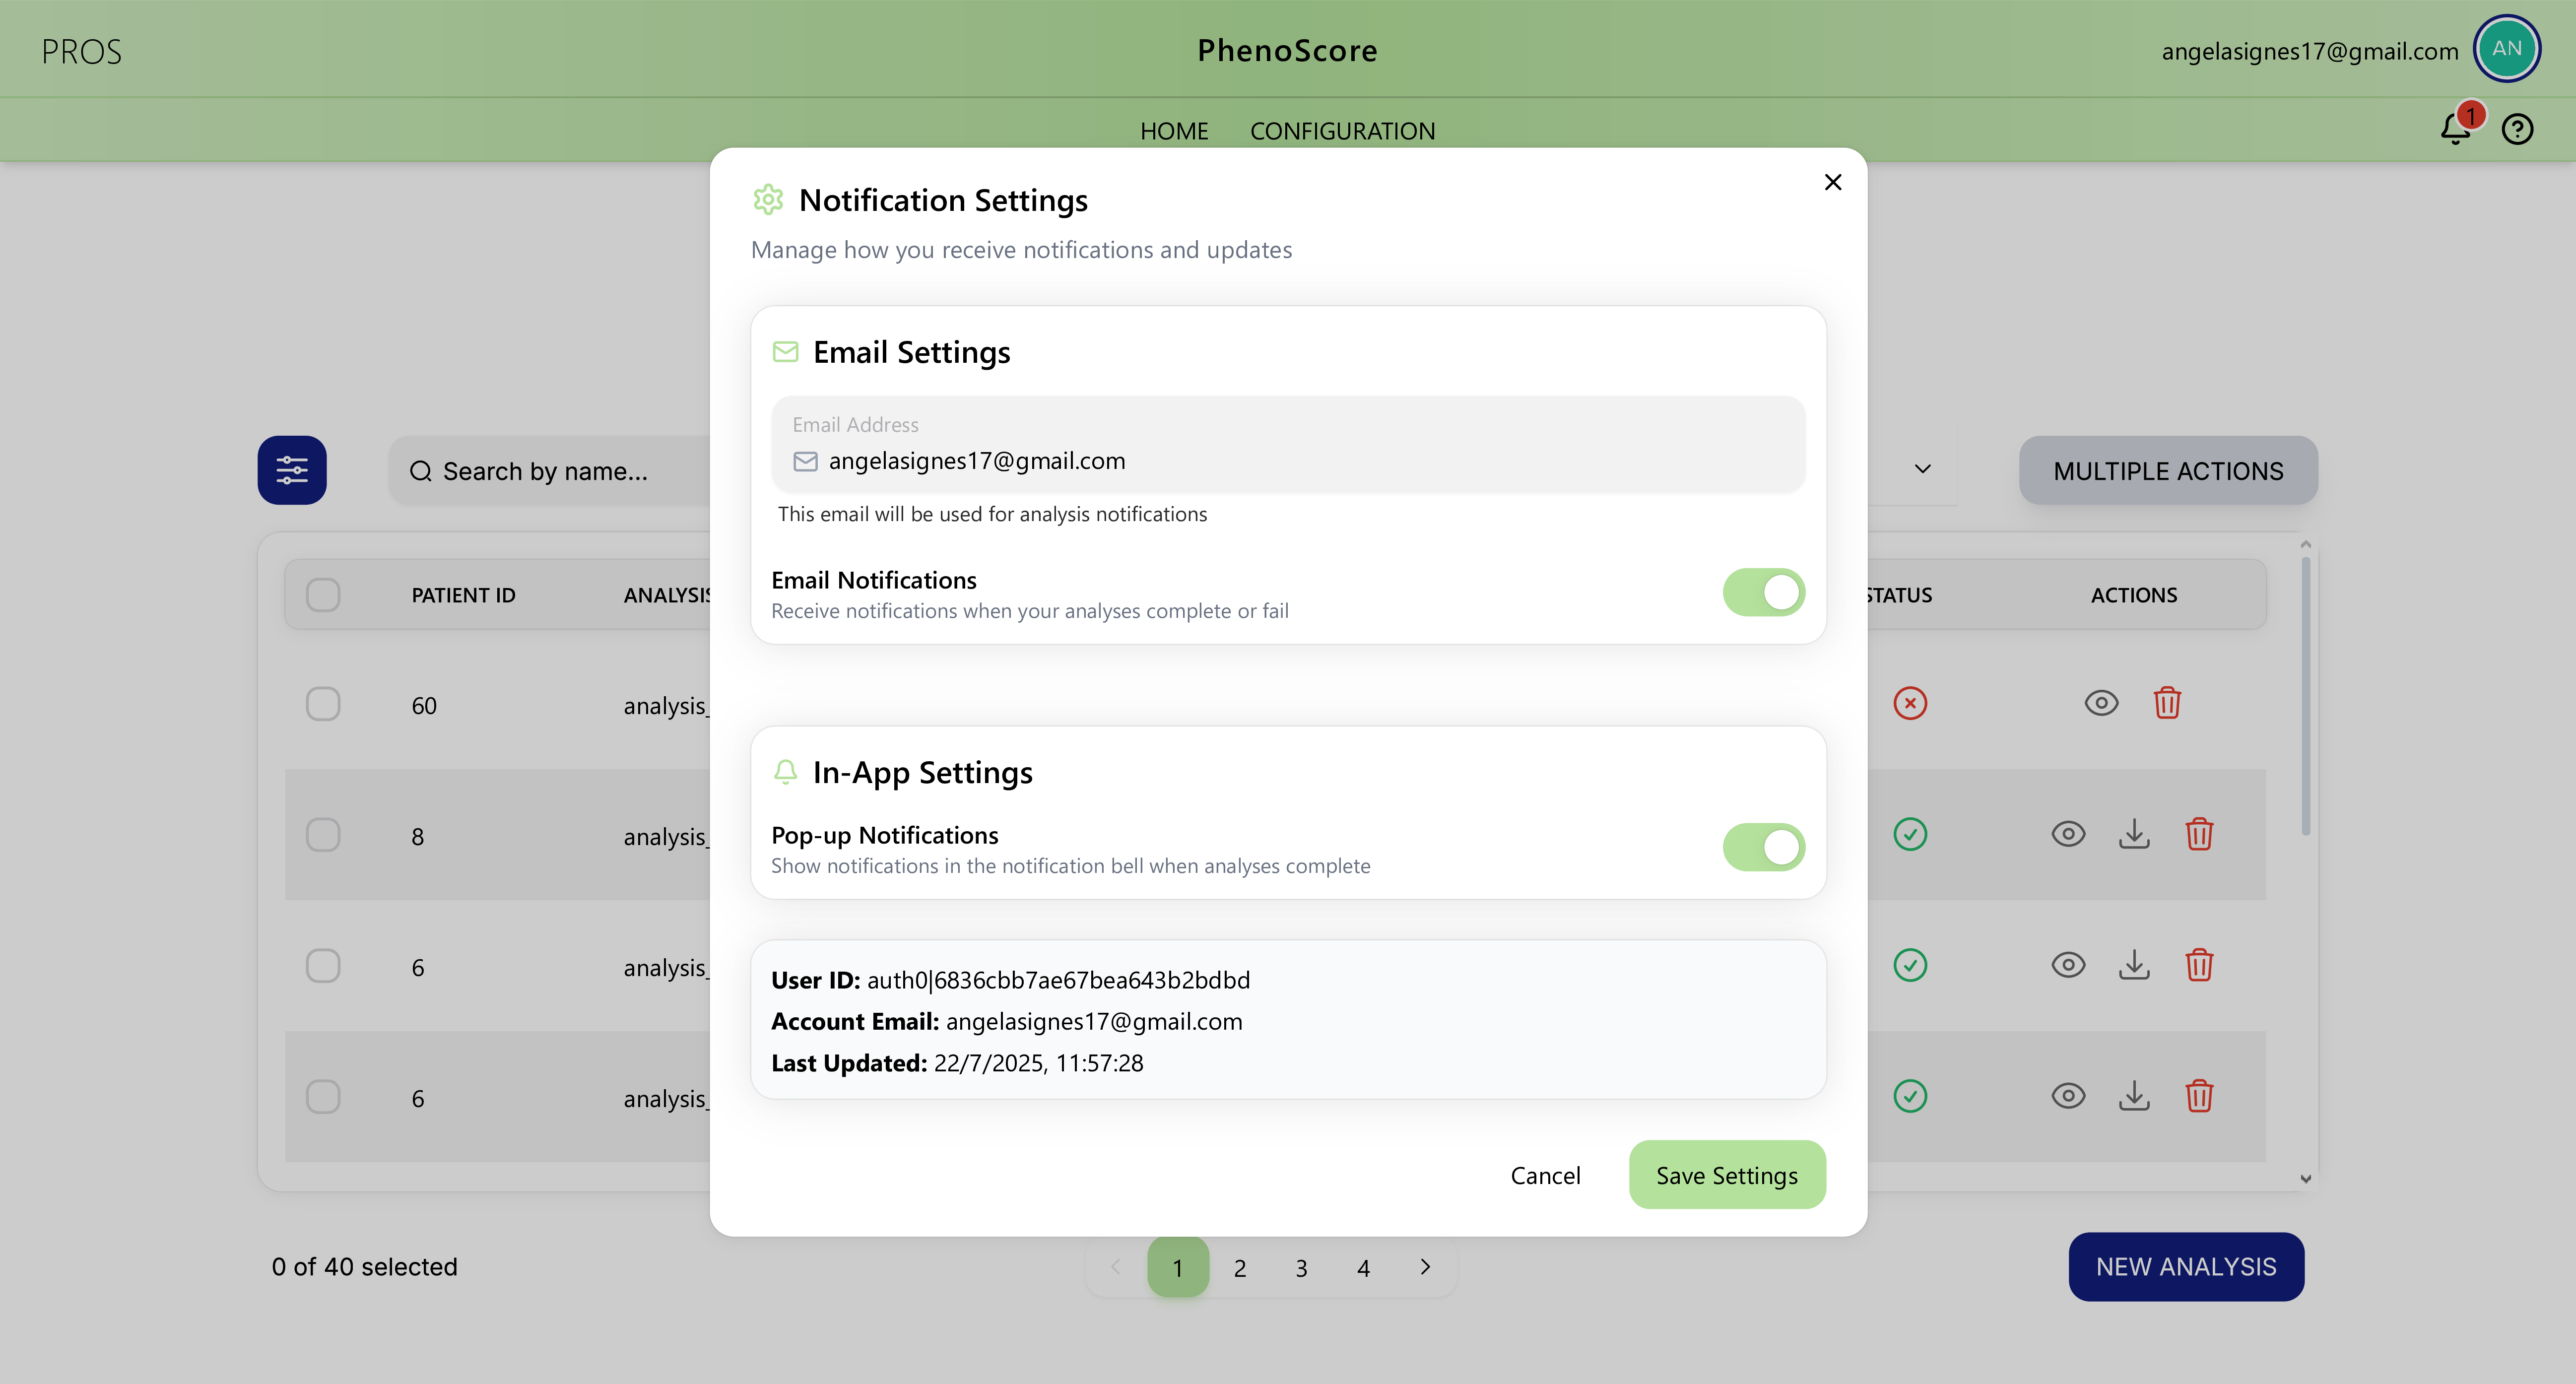
\includegraphics[width=1\textwidth]{tfgetsinf/images/Phenoscore-notifications.png}
    \caption{UI Configuración de las notificaciones}
    \label{fig:UINotificaciones}
\end{figure}

\subsubsection{Gestión de tareas asíncronas en la interfaz}

Con el objetivo de proporcionar una experiencia dinámica y ágil al usuario ante un sistema de \texttt{backend} asíncrono, la lógica completa del lado del cliente se encuentra encapsulada en un \textit{hook} personalizado de \textit{React}, \texttt{useLongAnalysis}. Este \textit{hook} se encarga de gestionar un ciclo de vida completo de un análisis, desde su creación y seguimiento hasta la actualización de los datos en tiempo real de la interfaz.

Su funcionamiento es el siguiente:

\begin{itemize}
    \item \textbf{Creación del Análisis:} Cuando el usuario envía el formulario de configuración, el \textit{hook} cambia a un estado de carga (\texttt{creatingAnalysis}) para dar un \textit{feedback} visual inmediato (por ejemplo deshabilitar el botón de envío). Hace una petición \texttt{POST} a \texttt{/api/analysis} con todos los datos del análisis y el identificador del usuario que ha extraído de \textit{Auth0}. El servidor acepta la petición inmediatamente confirmando que se ha encolado el trabajo, y en ese momento el \textit{hook} actualiza la lista general de análisis.
    \item \textbf{Monitorización del Estado mediante un Sistema de \textit{Polling Dual}:} Para mantener la interfaz sincronizada con el estado real del \texttt{backend}, el \textit{hook} implementa dos estrategias de \textit{polling} complementarias:
    \begin{enumerate}
        \item \textbf{\textit{Polling} Específico (Rápido):} Cuando el usuario interactúa con un análisis en particular, se activa una función de \textit{polling} recursiva que consulta el \textit{endpoint} \texttt{/api/status?id=\{analysisId\}} cada 2 segundos. Este \textit{polling} se detiene automáticamente en cuanto el estado del análisis deja de ser \textit{running}, asegurando una actualización casi en tiempo real con un uso eficiente de los recursos.
        \item \textbf{\textit{Polling} General (Lento):} De forma paralela, un intervalo global se ejecuta cada 5 segundos para llamar a la función \texttt{fetchAnalyses}. Esto garantiza que la lista principal de análisis esté siempre actualizada, reflejando el progreso de trabajos que puedan haber finalizado en segundo plano, en otra pestaña del navegador o incluso en otro dispositivo.
    \end{enumerate}
    \item \textbf{Actualización Reactiva de la Interfaz:} El \textit{hook} utiliza el sistema de estado de \textit{React} (\texttt{useState}) para almacenar la lista completa de análisis y el estado del análisis actualmente monitorizado. Cualquier cambio obtenido a través del \textit{polling} actualiza estos estados, lo que provoca que los componentes de la interfaz que los utilizan se re-rendericen automáticamente, mostrando al usuario la información más reciente sin necesidad de recargar la página.
    
    \item \textbf{Integración con la Seguridad:} La comunicación con la API está protegida por diseño. El \textit{hook} depende del estado de autenticación de \textit{Auth0} y no realiza ninguna petición si el usuario no está validado. El identificador único del usuario (\texttt{user.sub}) se adjunta a todas las llamadas a la API, permitiendo al \texttt{backend} filtrar y devolver únicamente los datos que pertenecen a dicho usuario.
\end{itemize}

Esta arquitectura, centrada en un \textit{hook} centralizado, no solo permite una experiencia de usuario eficiente y fluida, sino que también favorece un código más modular, reutilizable y sencillo de mantener, a la vez que sigue las buenas prácticas en cuanto a seguridad y rendimiento.


\subsection{Implementación de la capa de lógica de negocio (\texttt{backend})}
\label{subsec:desarrollo_backend}
El \texttt{backend} es el núcleo funcional de la aplicación. Se encarga de la lógica de negocio, la coordinación de tareas complejas y la comunicación segura con los servicios externos.

\subsubsection{Implementación de la API}
La comunicación entre el \texttt{frontend} y el \texttt{backend} se realiza a través de una API \textit{RESTful}.

En esta sección se explican detalladamente los \textit{endpoints} de la API desarrollada, incluyendo las rutas disponibles, sus funciones específicas y los métodos \textit{HTTP} implementados. La API gestiona todas las operaciones desde la carga de archivos, pasando por la creación y gestión de análisis, hasta la consulta de estados y resultados.

\begin{itemize}
    \item \textbf{\texttt{POST /api/upload}}: Este \textit{endpoint} permite subir archivos de pacientes y población de referencia al servidor. El proceso incluye: guardar el archivo del paciente (descomprimiendo si es \textit{.zip}), almacenar el archivo de población en la ruta correspondiente (o usar el \textit{path} fijo de 1000G si no se proporciona), registrar los datos en la base de datos y devolver un \textit{JSON} con los \textit{IDs} creados.
    \item \textbf{\texttt{/api/analysis}}:
        \begin{itemize}
            \item \textbf{\texttt{GET}}: Devuelve todos los análisis ordenados por fecha descendente, incluyendo información del paciente, población de referencia y modelos priorizados asociados.
            \item \textbf{\texttt{POST}}: Crea un nuevo análisis y lo añade a la cola de \textit{BullMQ} para procesamiento en segundo plano. Recibe un \textit{JSON} con los datos del análisis y devuelve el ID creado junto con una URL para consultar el estado.
            \item \textbf{\texttt{DELETE}}: Elimina un análisis específico. Requiere el parámetro \texttt{id} en la \textit{query string} y confirma la operación mediante \textit{JSON}.
        \end{itemize}
        
    \item \textbf{\texttt{POST /api/analysis/cancel}}: Cancela un análisis en curso, actualizando su estado a '\textit{failed}' y marcando el resultado \textit{HTML} como '\textit{aborted}'. Recibe el ID del análisis vía \textit{JSON} y confirma la operación exitosa.
    
    \item \textbf{\texttt{GET /api/analysis-details}}: Obtiene los detalles completos del análisis, es decir su configuración y otra información ligada a este, como la poblacion de referencia o los modelos PRS.

    \item \textbf{\texttt{POST /api/notifications/email}}: Manda un email al usuario cuando un análisis se ha ejecutado exitosamente o cuando ha fallado, adjuntando al correo el informe o el error detallado respectivamente.
    
    \item \textbf{\texttt{/api/notifications/read}}:
        \begin{itemize}
            \item \textbf{\texttt{GET}}: Obtiene todas las notificaciones que no han sido leídas aún por el usuario y las devuelve a la lista.
            \item \textbf{\texttt{POST}}: Marca una notificación como leída y por lo tanto ya no vuelve a aparecer en la lista de notificaciones.
            \item \textbf{\texttt{DELETE}}: Marca todas las notificaciones como leídas y la lista se queda vacía.
        \end{itemize}
        
    \item \textbf{\texttt{/api/notifications/settings}}:
        \begin{itemize}
            \item \textbf{\texttt{GET}}: Obtiene la configuración de las notificaciones del usuario.
            \item \textbf{\texttt{POST}}: Almacena una nueva configuración de notificaciones.
        \end{itemize}

    \item \textbf{\texttt{/api/queue}}:
        \begin{itemize}
            \item \textbf{\texttt{GET}}: Devuelve la información del estado de la cola como los trabajos del usuario que se están ejecutando
            \item \textbf{\texttt{POST}}: Se constituye por varias gestiones de la cola como la limpieza de trabajos antiguos o problemáticos.
        \end{itemize}
    
    \item \textbf{\texttt{GET /api/status}}: Consulta el estado de un análisis específico mediante el parámetro \texttt{id} en la \textit{query string}. Devuelve el análisis completo o un error si no existe.

    \item \textbf{\texttt{POST /api/upload}}: Recibe archivos de pacientes y poblaciones de referencia, se procesan y preparan para formar parte de la ejecución de los análisis.
\end{itemize}

\subsubsection{Ejecución asíncrona de los análisis PRS}

La ejecución de un análisis de Puntuación de Riesgo Poligénico (PRS) es la funcionalidad central de la aplicación y, debido a su complejidad, puede tardar hasta 25 minutos en ejecutarse. Por tanto, en vez de ejecutarlo de forma síncrona en el hilo principal porque bloquearía por completo la aplicación, se ha optado por diseñar una arquitectura asíncrona robusta basada en un sistema de colas y procesos de trabajo, cuya implementación y desafíos se detallan a continuación.\\

\textbf{Arquitectura asíncrona: Gestor de Cola y Procesador de Análisis}

La arquitectura se divide en dos componentes principales que colaboran para ejecutar los análisis de forma desacoplada:

\begin{itemize}
\item \textbf{Gestor de Trabajos (\texttt{AutoWorker}):} Este componente actúa como el intermediario entre la cola de trabajos y el procesador de análisis. Su responsabilidad es exclusivamente la gestión de la cola. Está orquestado por \textit{BullMQ}, un sistema de colas que utiliza \texttt{Redis} como intermediario de mensajería. Para asegurar la seguridad y flexibilidad, la conexión con \texttt{Redis} se configura mediante variables de entorno externalizadas. Cuando un nuevo trabajo de análisis es añadido a la cola por la API, el \texttt{AutoWorker} lo recoge y delega su ejecución al \texttt{AnalysisProcessor}. Esta capa de gestión también se encarga de la fiabilidad del sistema, configurando políticas de reintentos con un tiempo de espera exponencial para manejar fallos temporales sin sobrecargar el sistema.

\item \textbf{Procesador de Análisis (\texttt{AnalysisProcessor}):}
Este servicio, implementado en \\ \texttt{services/analysisProcessor.ts}, es el corazón de la lógica de procesamiento de los análisis genéticos. No sabe nada sobre el sistema de colas; su único propósito es recibir los datos de un análisis y ejecutarlo. El proceso que sigue es el siguiente:
\begin{enumerate}
    \item \textbf{Recuperación del Contexto:} Al recibir un trabajo, lo primero que hace es realizar una consulta completa a la base de datos para obtener todos los detalles del análisis: parámetros, datos del paciente, población de referencia y los modelos PRS seleccionados.
    \item \textbf{Preparación del Entorno:} Crea un directorio de ejecución único para el análisis y, dentro de este, genera los ficheros de configuración que la herramienta \textit{GenoPred} necesita como entrada: el fichero \texttt{score\_list.txt} (que lista los modelos a usar), el fichero \texttt{target\_list.txt} (que define la ruta al fichero del paciente y el formato del mismo) y el fichero \texttt{config.yaml} (que construye la entrada para el \textit{pipeline} \textit{Snakemake}). Para aportar flexibilidad, la localización de los ficheros de genotipado se gestiona de forma dinámica, permitiendo que la estructura de carpetas de entrada sea variable.
    \item \textbf{Invocación del Proceso Externo:} Utiliza el módulo \texttt{child\_process} de \textit{Node.js} para invocar el comando de ejecución del \textit{pipeline} de \textit{GenoPred}, activando primero el entorno \textit{Conda} necesario. Mientras el \textit{pipeline} se ejecuta, el procesador monitoriza la salida y actualiza el estado del análisis en la base de datos.
    \item \textbf{Gestión del Resultado:} Si se finaliza con éxito el trabajo, el procesador recupera el \textit{HTML} resultante, actualiza el estado de la base de datos a 'completado' y guarda la ruta al archivo \textit{HTML} para verlo más tarde.  En caso de un fallo, captura el error, lo registra y actualiza el estado a 'fallido'.
    \item \textbf{Cierre Seguro:} El procesador implementa un mecanismo de apagado seguro (\textit{graceful shutdown}).  Escucha las señales del sistema (como una orden de apagado) y cierra las conexiones a \texttt{Redis} y \texttt{Prisma} de manera segura para evitar la corrupción de datos y asegurarse de que no quede ningún trabajo pendiente en estado inconsciente.
\end{enumerate}
\end{itemize}
Tal separación de responsabilidades entre el gestor de colas y el procesador de análisis conduce a un diseño mucho más claro y mantenible. \texttt{AutoWorker} se encarga de la infraestructura de mensajería, dejando que \texttt{AnalysisProcessor} se concentre únicamente en la lógica de negocio relacionada con el análisis bioinformático, resolviendo así el gran desafío de ejecutar procesos pesados sin bloquear la aplicación y de manera modular.

\textbf{Desafíos en la Implementación del \textit{Worker}}

Mientras se estaba llevando a cabo la implementación del \textit{worker}, hubo varios desafíos que requirieron replantear la arquitectura de despliegue, además de realizar cambios a causa de un error del cual no se encontraba la causa. 

El primer obstáculo surgió al elegir el entorno de ejecución basado en \textit{Windows}, usando el subsistema de \textit{Windows} para \textit{Linux (WSL)}, para la ejecución de la \textit{pipeline} \textit{GenoPred}. Esta arquitectura llevó a desarrollar una lógica específica para la traducción de rutas de ficheros al formato \textit{Linux}, lo cual fue indispensable para que el \textit{pipeline} localizara los datos necesarios. 

Por otra parte, en el inicio se planteó la posibilidad de cambiar uno de los parámetros de la configuración del análisis, el '\textit{overlap threshold}', el cual se refiere al porcentaje de coincidencia entre las variantes genéticas (SNPs) que aparecen en el archivo de puntuación PGS y las variantes que existen en los datos de referencia de \textit{GenoPred}. Si este porcentaje es menor del 75\% se descarta el archivo y no se calcula la puntuación para esa muestra. Posteriormente, se tuvo que descartar la idea de poder variar este parámetro, ya que en el \textit{pipeline} no se ha considerado esa opción, por lo tanto no solo depende de los ficheros de entrada sino que se tendría que cambiar también el código interno de la herramienta, lo cual no entra dentro de las posibilidades del proyecto. 

Un mayor imprevisto surgió tras una actualización del \textit{pipeline} \textit{GenoPred}, ya que la nueva versión introdujo cambios que rompían con la anterior compatibilidad, dando un aviso de error relacionado con el reporte individual de puntuación poligénica. Al intentar reinstalar la herramienta con sus nuevas dependencias, el entorno \textit{WSL} empezó a dar errores fatales, impidiendo seguir con el desarrollo de la aplicación; ante este percance se tomó la decisión de migrar todo el entorno a una máquina virtual con un sistema operativo \textit{Linux}. Este cambio proporcionó un entorno más robusto y predecible. 

A pesar de la estabilidad ganada con el nuevo entorno, los análisis seguían fallando debido al \textit{bug} introducido en \textit{GenoPred}. Tras depurar el análisis y recurrir a la documentación, se tomó la decisión de contactar directamente con el desarrollador principal de la herramienta. Su colaboración fue fundamental; amablemente confirmó la existencia del \textit{bug} en la nueva versión e introdujo unos nuevos cambios libres de errores de código. Gracias a estos, el problema se resolvió y los análisis se volvieron a ejecutar correctamente.

Por último, se tomó la decisión de realizar una última migración, el despliegue de la solución en una máquina virtual en la nube a través de \textit{Google Cloud Platform (GCP)}, para facilitar en un futuro la puesta en producción de la herramienta, garantizando así la escalabilidad y disponibilidad del servicio que se busca proporcionar desde un inicio. 

\subsubsection{Gestión de autenticación y seguridad}
Para la gestión de la autenticación y la autorización de usuarios, se ha integrado el servicio externo \textit{Auth0}. Esta decisión delega la responsabilidad de gestionar contraseñas, sesiones y \textit{cookies} a un proveedor especializado, lo que resulta en una solución más segura y robusta que una implementación propia. \textit{Auth0} proporciona, además, funcionalidades avanzadas como el inicio de sesión a través de redes sociales.

\subsection{Implementación de la capa de datos y persistencia}
\label{subsec:desarrollo_datos}
Esta capa es la responsable de la interacción con la base de datos y el almacenamiento en memoria.

Para la gestión de los datos relacionales, se ha utilizado \texttt{Prisma}, un \textit{ORM (Object-Relational Mapping)} de nueva generación. \texttt{Prisma} permite definir el esquema de la base de datos de forma tipada en el fichero \texttt{schema.prisma}, facilitando las migraciones y generando un cliente seguro para realizar consultas, lo que reduce drásticamente la posibilidad de errores en la interacción con la base de datos.

Para la gestión de la cola de trabajos asíncronos, se ha utilizado \texttt{Redis}, una base de datos en memoria que actúa como intermediario de mensajes para \textit{BullMQ}. Su alta velocidad es ideal para gestionar el estado de las colas de manera eficiente.